\documentclass[12pt,a4paper,ruledheader,tocpage=prefix,floatnumber=continuous,pagestart=folhaderosto,font=times]{abnt}
\usepackage[top=3cm,left=3cm,right=2cm,bottom=2cm]{geometry}

\usepackage[utf8]{inputenc}
\usepackage{fancyhdr}
\usepackage{enumerate}
\usepackage{array}
\usepackage[table]{xcolor}
\usepackage{listings}
\usepackage[brazil]{babel}
\usepackage{graphicx}
\usepackage{float}
% – inicio codigo fonte
\usepackage{listings}
\usepackage{xcolor}
\newcommand{\listofcodename}{Lista de Códigos}
%% Abrevia figuras e tabelas
\def\figurename{Fig.}
\def\tablename{Tab.}

%opening

\begin{document}
%capa
%%%%%%%%%%%%%%%%%%%%%%%%%%%%%%%%%%%%%
%% Capa
%%%%%%%%%%%%%%%%%%%%%%%%%%%%%%%%%%%%%

\thispagestyle{empty}

\begin{titlepage}
 \vfill
 \begin{center}

	\begin{figure}[htb]
		\centering 
\includegraphics[scale=1]{preTextuais/img/uel.png}
	\end{figure}

	\begin{figure}[htb]
		\centering 
\includegraphics[scale=.67]{preTextuais/img/barra_capa.png}
	\end{figure}
	
	
	{\large Departamento de Computa\c{c}\~ao \\
	Trabalho de Conclus\~ao de Curso}

	\vspace*{\stretch{4}}
	{\large \textbf{ANA CAROLINA ALVES RODRIGUES}}

	\vspace*{\stretch{4}}
	{\Large \textbf{GEST\~AO DE PORTF\'OLIO DE PROJETOS}}

	\vspace*{\stretch{7}}

	\begin{figure}[htb]
		\centering 
\includegraphics[scale=.67]{preTextuais/img/barra_capa.png}
	\end{figure}
	\vfill
	{\bf Londrina \\
 	2012}
	\end{center}
\end{titlepage}



%folharosto
%%%%%%%%%%%%%%%%%%%%%%%%%%%%%%%%%%%%%
%% Folharosto
%%%%%%%%%%%%%%%%%%%%%%%%%%%%%%%%%%%%%

%% n�o numerar a p�gina
\thispagestyle{empty}


\begin{center}
{\large ANA CAROLINA ALVES RODRIGUES}

\vspace{1.6in}
{\Large \textbf{GEST\~AO DE PORTF\'OLIO DE PROJETOS}} 

\vspace{2.0in}
\begin{flushright}
\parbox{3.2in}{Trabalho de Conclusao de Curso apresentado ao Curso de Graduacao em Ciencia da Computacao
da Universidade Estadual de Londrina, como requisito parcial a obtencao do grau de Bacharel.}
\end{flushright}
 
\vspace{0.5in}
\begin{flushright}
\parbox{3.2in}{
Orientador: Prof. Dr. Rodolfo Miranda de Barros.}
\end{flushright}
  
\vspace{1.2in}
\begin{center}
{\bf Londrina \\
 2012}
\end{center}
\end{center}
% \folhaderosto

%aprovacao
%%%%%%%%%%%%%%%%%%%%%%%%%%%%%%%%%%%%%
%% Folha de Aprovacao
%%%%%%%%%%%%%%%%%%%%%%%%%%%%%%%%%%%%%

%% n�o numerar a p�gina
\thispagestyle{empty}

\begin{center}
{\large ANA CAROLINA ALVES RODRIGUES}

\vspace{0.9in}
{\Large \textbf{GEST\~AO DE PORTF\'OLIO DE PROJETOS}}

\vspace{1.3in}
\begin{flushright}
\parbox{3.0in}{
Trabalho de Conclus\~{a}o de Curso apresentado ao Curso de Gradua\c{c}\~{a}o em Ci\^{e}ncia da Computa\c{c}\~{a}o
da Universidade Estadual de Londrina, como requisito parcial a obten\c{c}\~ao do grau de Bacharel.}
\end{flushright}

%\vspace{0.5in}
%\begin{flushright}
%\parbox{3.0in}{
%Orientador: Dra. Jandira Guenka Palma}
%\end{flushright}

\vspace{0.5in}
\begin{flushright}
	\begin{tabular}{c}
		\hline
		Prof. Dr. Rodolfo Miranda de Barros \\
		Universidade Estadual de Londrina - UEL
		\\
		\\
		\\
		\hline
		Prof\textordfeminine. Dr\textordfeminine. Jandira Guenka Palma \\
		Universidade Estadual de Londrina - UEL
		\\
		\\
		\\
		\hline
		Prof. Msc. Rafael Robson Negr\~{a}o \\
		Universidade Estadual de Londrina - UEL
		\\
		\\
		\\
		
		Londrina, \rule{20pt}{1pt} de Novembro de 2012
		
	\end{tabular}
\end{flushright}
\end{center}




%dedicatoria
\
\vfill

\begin{flushright}
\hfill \textit{\`{A} minha mãe, pelo amor incondicional e motivação diária.}
\end{flushright}

\vspace*{1cm}

\clearpage

%agradecimentos
\chapter*{Agradecimentos}
\begin{trivlist}  \itemsep 2ex  \normalsize
	\item � Deus pelo desafio da vida.
	\item Aos amigos e amigas, pelos bons e maus momentos, ``fitas erradas'' e principalmente pela amizade.
 
  \item \`{A} falta de dinheiro, por n\~{a}o me fazer desistir.

% \item \`{A} m\'{u}sica pelo que ela \'{e} capaz.

 \item \`{A} todos os professores e funcionarios do departamento de computacao que ajudaram a
 concluir a minha graduacao em Ciencia da Computacao.
\item Ao Coringa por seu esp\'{\i}rito de vida inspirador.
\item Ao \'{a}lcool, a cafe\'{\i}na e a pizza por diversos momentos.
\end{trivlist}

%epigrafe
\
\vfill

\begin{flushright}
\hfill \textit{``Essencialmente, todos os modelos estao errados, mas alguns sao uteis.''.} \\
{\bf George Box}
\end{flushright}

\begin{flushright}
\hfill \textit{``O gato ou o Quico?''.} \\
{\bf Chaves}
\end{flushright}

\vspace*{1cm}



%resumo e abastrac
\singlespacing
\noindent ALVES RODRIGUES,  Ana Carolina  {\bf Gest\~ao de Porftolio de Projetos}. 2012. 85 f. TCC - Universidade Estadual de Londrina, Londrina. 2012. \\
\begin{center}
{\bf {\Large RESUMO}}
\end{center}
Texto do resumo 
\newline

\noindent{\bf Palavras-Chave:}  palavra-chave1, palavra-chave2...palavra-chaven.
 
%%%%%%%%%%%%%%%%%%%%%%%%%%%%%%%%%%%%%%%%%%%%%%%%%%%%%%%%%%%%%%%%%%%%%%%%%%%%%%%%%
% fim de arquivo
%%%%%%%%%%%%%%%%%%%%%%%%%%%%%%%%%%%%%%%%%%%%%%%%%%%%%%%%%%%%%%%%%%%%%%%%%%%%%%%%%

\begin{abstract}
\vspace{1.5ex}

\textbf{Keywords:} 

\end{abstract}

\listadefiguras
\cleardoublepage 
\listadetabelas
\cleardoublepage
\chapter*{Lista de Siglas e Abreviaturas}

\noindent
% organize as siglas e abreviaturas em ordem alfab�tica
\begin{tabular}{l c p{.85\linewidth}}
	{\bf AHP}	&-	& Analytic Hierarchy Process \\
	{\bf CFO}	&-	& Chief Financial Officer \\
	{\bf CIO}	&-	& Chief Information Officer \\
	{\bf FCS}	&-	& Fatores Cr\'{i}ticos de sucesso \\
	{\bf GPP}	&-	& Gest\~{a}o de Portfolio de Projetos \\
	{\bf NPV}	&-	& Net Present Value \\
	{\bf PDCA}	&-	& Plan Do Check Act \\
	{\bf PMBOK}	&-	& A Guide to the Project Managemente Body of Knowledge \\
	{\bf PMI}	&-	& Project Management Institute \\
	{\bf PMO}	&-	& Project Management Office \\
	{\bf PO}	&-	& Project Office \\
	{\bf PP}	&-	& Payback Period\\
	{\bf ROI}	&-	& Return on investment\\
	{\bf RONA}	&-	& Return on Net Assets\\
	{\bf TI}	&-	& Tecnologia da Informa\c{c}\~{a}o\\
	{\bf VPL}	&-	& Valor Presente L\'{i}quido\\
	{\bf WBS}	&-	& Work Breakdown Structure\\
\end{tabular}


\tableofcontents

\chapter{Introdução}
Atualmente o desenvolvimento de projetos tem buscado soluções que auxiliem a demanda do mercado de forma que seus recursos possam ser aplicados
consistentemente, fazendo assim com que os atrasos, desperdícios e prejuízos sejam minimizados. Para isso busca-se utilizar ferramentas e 
técnicas que contemplem aspectos de eficiência (uso de recursos) e eficácia (obtenção de resultados positivos para a organização).
Dessa forma torna-se comum a utilização de técnicas como gerência de projetos e gerência de portfolio, essa segunda ainda pouco utilizada no Brasil.

Enquanto o gerenciamento de projetos ou programas está interessado em soluções que ``façam certo o trabalho'', a gestão de portfolio visa o ``faça o 
trabalho certo''.\cite{sppm} De forma a orientar a escolha pelos projetos que sejam mais viáveis para a empresa em relação as metas estratégicas 
existentes. 

No estudo ‘CHAOS Summary 2009’, o instituto de pesquisa Standish Group informa que houve uma queda nas taxas de sucesso dos projetos de TI. Pelo 
relatório, só 32\% das iniciativas são bem-sucedidas. Ou seja, 68\% das atividades programadas pelo CIO e sua equipe acabam não atingindo os objetivos.

O propósito do processo Gestão de Portfólio de Projetos é iniciar e manter projetos que sejam necessários, suficientes e sustentáveis, de forma a 
atender os objetivos estratégicos da organização, porém há pouco conhecimento sobre quais fatores da gestão de portfolio de projetos são específicos do 
contexto e quais são universais. Este processo compromete o investimento e os recursos organizacionais adequados e estabelece a autoridade necessária 
para executar os projetos selecionados.\cite{mps}

\section{Objetivos}
O objetivo principal deste trabalho esta pautado no estudo sobre Gestão de Portfólio de Projetos, para obtenção de conhecimento sobre quais são suas principais
vantagens e desafios. Bem como o conhecimento de modelos e ferramentas já existentes para a utilização dessa ferramenta. A partir de pesquisas no campo não
apenas da Gestão de Portfolio mas também da Gerência de Projetos e Estratégias Organizacionais.

Com tais conhecimentos, pretende-se a elaboração de um modelo próprio para a gestão. Capaz de atender as necessidades específicas das organizações desenvolvedoras
de software. Para que ao final seja possível o desenvolvimento uma ferramenta para que utilizando tal metodologia nestas organizações específicas.

Pretende-se desenvolver a ferramenta de forma que esta possa ser aplicada de forma satisfatória nas organizações, fazendo com que os gastos
empreendidos para o desenvolvimento de software fiquem abaixo das ganhos obtidos, tendo maior controle sobre a carteira de projetos será possível
equilibrar onde e quais recursos deverão ser utilizados e de que forma, aumentando assim a produtividade organizacional.

\section{Organização}
Este trabalho está dividido em seis capítulos. Este capítulo introdutório, que oferece informações sobre o propósito do trabalho e mais cinco.
O segundo capítulo diz respeito a estratégia organizacional, onde serão apresentados conceitos importantes para tratar da Gestão de Portfólio e como estes
devem ser trabalhados dentro da organização para garantir a gestão.

O terceiro capítulo apresenta informações sobre o gerenciamento de projetos, suas definições e propriedades necessárias para sua utilização dentro das 
organizações. O quarto capítulo trata da Gestão de Portfolio em si. Serão apresentados as informações inerentes a ela, bem como os principais fatores para sua
garantia. Além de informações sobre seus benefícios e desafios.

O quinto capítulo apresenta os principais modelos de Gestão de Portfolio estudados. O sexto capítulo apresenta as considerações finais do trabalho e as lições
aprendidas através deste.

\chapter{Estratégia Organizacional}
Segundo Prahalad (1997), a estratégia organizacional deve ter como ponto central o intuito de desenvolver uma série de competências essenciais, e partindo
disso, criar novos produtos e serviços. Tal processo exige que exista uma nova forma de pensar por parte da organização, o que o autor descreve como um
``desaprendizado'' ou readaptação por parte dos dirigentes. 

Toda empresa possui o desejo de possuir estratégias que serão responsáveis pelas mudanças no cenário atual e assim pelo que existirá no futuro. Para que possam
criar tais estratégias, que não sejam apenas um exercício de posicionamento, é necessário que tal processo seja diferenciado. Isto é, não deve-se buscar 
compreender o que já existe e como é feito, mas descobrir como é possível a criação de novas atividades, empreendimentos e negócios. 

A partir dessa perspectiva, Prahalad (1998), aponta que a estratégia não deve ser apenas um exercício de analisar as atividades já realizadas e sim um processo
de descoberta. Assim, a partir daí a estratégia passa a ser inovação e criatividade: tornando-se a busca por novas oportunidades e interação entre clientes, 
empresas, tecnologias e mercado.

Os meios para que seja possível atingir as metas e critérios traçados pela alta administração da organização são as estratégias, e essas
podem ser classificadas em quatro tipos distintos: sobrevivência, manutenção, desenvolvimento e crescimento. Onde cabe a administração a determinação do conjunto
de estratégias que será adotado, de forma que os aspectos gerais não acabem gerando conflitos entre si.

Os níves de planejamento diferenciam-se de acordo com seu significado, alcance ou impacto, definindo assim o ato de planejar em si. Podemos dividir o 
planejamento em três níveis\cite{sanvicente}:

\begin{itemize}
 \item Planejamento estratégico: onde as decisões a serem tomadas deverão dizer respeito principalmente aos problemas externos da empresa, onde veremos geralmente
       problemas ligados às linhas de produtos e serviços e os mercados atendidos.
 \item Planejamento administrativo: aqui a preocupação estará voltada para a melhor estruturação possível dos recursos (humanos, físicos e financeiros).
 \item Planejamento operacional: as atividades previstas buscam a utilização dos recursos de forma mais eficiente para um determinado período de tempo.
\end{itemize}

Segundo Kaplan (2000), as estratégias dizem respeito ao item mais importante do planejamento estratégico das organizações, pois é através da estratégia
que os executivos possuem o poder de mudar o rumo da organização. Porém, não é correto dizer que esse seja o fator único e determinante para o sucesso ou
fracasso da mesma. A competência da cúpula administrativa é tão importante quanto uma boa estratégia. E deverá estar focada na satisfação da necessidade
dos clientes.

\section{Planejamento Estratégico}
O planejamento estratégico de uma organização tem como intuito definir objetivos para a seleção de programas de ação e execução, levando em conta as 
condições internas e externas inerentes a instituição e a evolução almejada.No planejamento são definidos para que setores serão distribuídos os recursos 
existentes, de forma que os objetivos e metas traçadas sejam alcançados ao longo do processo. 

\begin{flushright}
 \hfill \textit{``[...] são pré-requisitos a clara definição da missão da empresa, envolvimento e a participação dos gestores, e o apoio de sistema de 
informações sobre variáveis ambientais, que gerem informações sobre os desempenhos passados e propiciem o conhecimento das variáveis atuais dos 
ambientes interno e externo`` (CATELLI, 1999, p.59).}
\end{flushright}

É um planejamento global a curto, médio e longo prazo, que também  considera premissas básicas que deverão ser respeitadas pela instituição para que o 
processo tenha coerência e sustentação. O planejamento estratégico deve comportar decisões sobre o futuro da organização, como:\cite{rodolfo} 

\begin{itemize}	
\item Objetivos organizacionais a longo prazo e seu desdobramento em objetivos departamentais detalhados; 
\item As atividades escolhidas, isto é, os produtos (bens ou serviços) que a organização pretende produzir;
\item O mercado visado pela organização, ou seja, os consumidores ou clientes que ela pretende abranger com seus produtos;
\item Os lucros esperados para cada uma de suas atividades;
\item Alternativas estratégicas quanto às suas atividades (manter o produto atual, maior penetração no mercado atual, desenvolver novos mercados);
\item Interação vertical em direção aos fornecedores de recursos ou integração horizontal em direção aos consumidores ou clientes;
\item Novos investimentos em recursos (materiais, financeiros, máquinas e equipamentos, recursos humanos, tecnologia etc.) para inovação (mudanças) ou para crescimento (expansão).
\end{itemize}

Ao término do planejamento estratégico a organização deve possuir missão, visão e valores bem definidos, a partir daí os projetos e processos da mesma
deverão ser desenvolvidos de acordo com estas definições, para que os objetivos e metas traçados possam ser alcançados e o planejamento bem sucedido.

Existe uma estimativa de que entre as 500 maiores empresas do mundo listadas pela Fortune de 50\% a 75\% delas têm suas principais estratégias ancoradas 
em projetos de TI.O que evidencia a necessidade de técnicas e ferramentas que possam culminar no sucesso de tais estratégias.

Deve-se lembrar que o planejamento é um processo contínuo, no qual estão envolvidas de forma simultânea a formulação, implementação e reformulação da
estratégia. Assim é possível verificar de forma evidente que a implementação da estratégia retroalimenta o processo do planejamento estratégico em si, 
e em alguns casos é possível que os dois acabem por se confundir. Reforçando assim a importância da existência de uma implementação plena, como uma forma
de assegurar a melhora da própria estratégia.

\chapter{Gerenciamento de projetos}
Podemos considerar que projetos são semelhantes à operações, por serem executados por pessoas e, geralmente apresentarem limitações referentes a recursos e
serem planejados, executados e controlados. O que difere entre estes é principalmente o fato de as operações possuírem um caráter contínuo e repetitivo, ao
passo em que os projetos têm um caráter temporário e exclusivo \cite{sppm}.

Podemos considerar que existem duas grandes maneiras de se observar o gerenciamento de projetos. A primeira e mais antiga, esta baseada no conceito de 
ciclo de vida do projeto e também possui parte de uma premissa temporal, onde o projeto será dividido em fases. Sendo essas: concepção, planejamento,
execução e fechamento.

Já a segunda, diz respeito a metodologia difundida pelo PMI – Project Management Institute, que surgiu no início dos anos 90 e hoje apresenta-se como
referência no assunto. Esta parte do pressuposto que existem diversas disciplinas que necessitam ser aplicadas aos projetos para assegurar seu sucesso.

Tais disciplinas, descritas em detalhes no PMBOOK (2008) ( A Guide to the Project Managemente Body of Knowledge), são: gerenciar prazo, gerenciar custo,
gerenciar qualidade, gerenciar escopo, gerenciar risco, gerenciar comunicação, gerenciar recursos humanos, gerenciar suprimentos/contratação, assim como,
gerenciar integração (que inclui planejamento, acompanhamento e controle de mudanças).

Se observarmos de forma cuidadosa iremos perceber que as duas formas são bastante complementares. Pois a abordagem apresentada pelo PMI considera tanto
o aspecto de ciclo de vida do projeto quanto as suas disciplinas.

Atualmente, com as aceleradas mudanças no mundo dos negócios, as organizações encaram o desafio de ter de lidar com um gerenciamento de portfolios de projetos
ao invés de simples operações de hierarquia corporativa. Neste cenário, a gestão por projetos nas empresas mostra como será possível atingir as metas traçadas
aplicando técnicas de gerenciamento de projetos, não apenas individualmente, mas também no nível estratégico.

Segundo Dinsmore (1999, p.22), o gerenciamento por projeto traz consigo a pergunta ``Como podemos tornar o negócio mais adaptável, sensível e lucrativo
em um ambiente de múltiplos projetos, que muda rapidamente?'' em contraste com a gerência de projeto tradicional, que visa responder a pergunta ``Como
podemos conseguir que este projeto seja feito eficaz e eficientemente?''. Porém, deve-se observar que novamente, ambos são complementares e trabalham em
conjunto com o intuito de aumentar a produtividade e a eficácia da organização.

\begin{flushright}
\hfill \textit{“A estratégia de mudança e inovação das organizações é implementada 
através de projetos, a capacidade de implementar projetos com taxa de 
sucesso maior que seus concorrentes pode ser considerada uma 
competência essencial de uma organização como definido por Hamel \& Prahalad (1994)”. }
\end{flushright}

\section{Ciclo de vida do projeto}
O ciclo de vida do projeto é capaz de oferecer uma estrutura básica para que possa ser realizado o gerenciamento do projeto, o que será independente do trabalho
específico envolvido. Consiste em fases que geralmente são sequenciais e em determinadas ocasiões acabam por se sobrepôr, sendo que seu nome e quantidade 
são determinados pela necessidade apresentada pelo gerenciamento da organização, a natureza do projeto e sua àrea de aplicação.\cite{pmbok}

Podemos documentar um ciclo de vida como uma metodologia. Sendo que este pode ser definido ou moldado de acordo com os aspectos inerentes a organização.
Sabendo que projetos possuem início e fim bem definidos, a variação das entregas e atividades específicas poderão ser grandes.

Projetos tendem a variar em tamanho e complexidade. Porém, não importa se estes são grandes, simples ou complexos. É possível que sejam mapeados para uma
estrutura básica de ciclo de vida\cite{pmbok}:

\begin{itemize}
 \item Início do projeto;
 \item Organização e preparação;
 \item Execução do trabalho do projeto e
 \item Encerramento do projeto.
\end{itemize}

A utilização dessa estrutura geralmente se dá no momento da comunicação com a alta administradação ou entidades que não estejam tão familiarizadas com detalhes
do projeto. Pois é uma visão de alto nível que oferece informações sobre o projeto sem oferecer grandes detalhes técnicos e pode ser utilizada em mais de uma
ocasião.

Segundo o \cite{pmbok} uma estrutura genérica do ciclo de vida em geral apresenta as seguinte características:

\begin{itemize}
 \item Níveis de custo e pessoal na fase inicial costumam ser baixos, e atingem um valor máximo durante a execução do projeto, e ao final do mesmo sofrem
       uma rápida queda.
 \item Durante o início do projeto é possível perceber uma maior influência das partes interessadas, bem como os riscos e incertezas.
 \item No início é evidente a capacidade de influenciar as características finais do projeto, sem que haja um impacto significativo sobre os custos, porém
       vai diminuindo conforme o projeto caminha para seu término. Na figura a seguir é possível perceber que os custos das mudanças e correções de erros
       apresentam aumento significativo conforme o projeto se aproxima do término.
\end{itemize}

\begin{figure}[H]
\centering
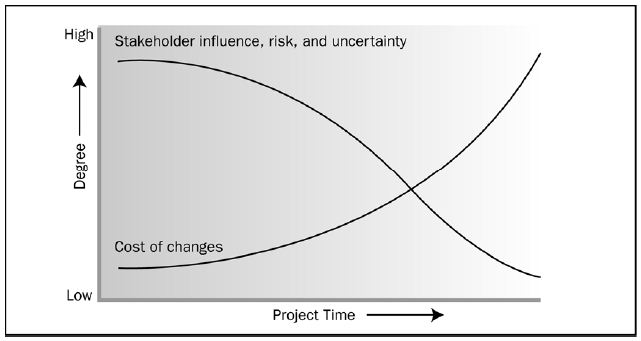
\includegraphics[width=.9\textwidth]{pmbok1.jpg}
\caption{Impacto da variável com base no tempo decorrido do projeto\cite{pmbok}.}
\end{figure}

Um gerente de projetos que esteja trabalhando dentro do contexto da estrutura genérica do ciclo de vida, poderá determinar que exista um controle maior 
sobre determinadas entregas. Geralmente projetos grandes e complexos requerem tal nível de controle. Nestas situações, o trabalho que deverá ser realizado
para atingir os objetivos traçados poderá se beneficiar com uma divisão formal de fases do projeto.  

\section{Processos de gerenciamento de projetos}
“Um processo é um conjunto de ações e atividades inter-relacionadas
realizadas para obter um conjunto pré-especificado de produtos, resultados ou serviços.”\cite{pmbok}

O objetivo do gerenciamento de projetos é que seja possível iniciar, planejar, executar, monitorar e controlar, e encerrar um projeto específico. E tem um
fator integrador que cria assim a necessidade de que cada processo estejam adequadamente associado e conectado a outros, para facilitar sua coordenação.

Para o PMBOK os processos de gerenciamento de projetos estão agrupados em termos da integração entre eles, das integrações existentes dentro deles e dos 
objetivos que estes devem alcançar. Tais processos estão agregados em cinco grupos, definidor como grupos de processos de gerenciamento de projetos. São eles:

\begin{itemize}
 \item Processos de iniciação: onde são definidos e autorizados os projetos ou fases deste.
 \item Processos de planejamento: responsáveis por definir e refinar os objetivos e planejar as ações necessárias para alcançar os objetivos e o escopo para
       os quais o projeto foi realizado.
 \item Processos de execução: onde é realizada a integração entre as pessoas e os demais recursos para que seja possível realizar o plano de gerenciamento do
       projeto.
 \item Processos de monitoramento e controle: mede e monitora regularmente o progresso, a fim de identificar variações em relação ao plano de gerenciamento do
       projeto, de forma que possam ser tomadas ações corretivas quando necessário para atender aos objetivos do projeto.
 \item Processos de encerramento: responsáveis por formalizar a aceitação do produto, serviço ou resultado e conduzir o projeto ou uma fase deste para um final
       ordenado.
\end{itemize}

A integração existente entre os processos apresentados acima pode ser melhor visualizada na imagem a seguir.

\begin{figure}[H]
\centering
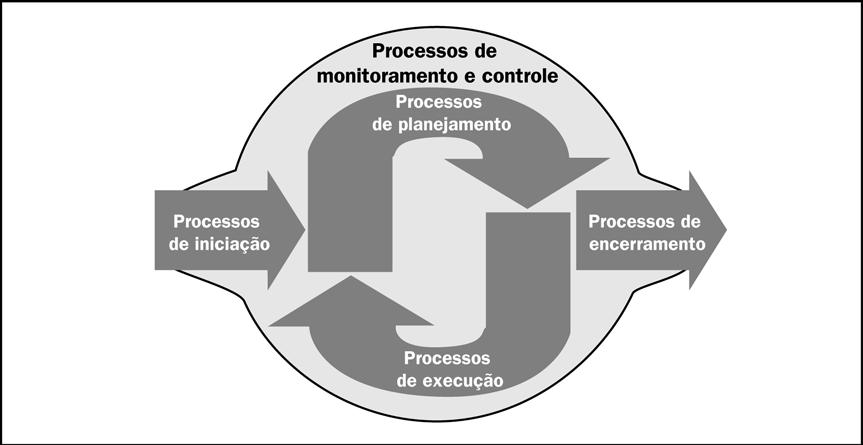
\includegraphics[width=.9\textwidth]{pmbok2.JPG}
\caption{Integração entre os processos de gerenciamento de projetos através de um ciclo do tipo PDCA.\cite{pmbok}.}
\end{figure}

\section{Project Management Office}
Para que seja possível controlar e gerenciar projetos de forma eficaz, faz-se necessário uma metodologia, organização e disciplina grande. As empresas 
atuais possuem grande volume de projetos, com diferentes níveis de complexidade. E cabe ao gerente de projetos conhecer e administrar de uma forma geral
cada um destes. Com o intuito de suprir esta demanda, as empresas estão optando cada vez mais pela utilização do conceito de Projeto Office – PO ou Project 
Management Office – PMO.
 
Este conceito diz respeito a área da empresa que possuirá uma visão holística dos projetos da mesma. Tendo conhecimento destes, o PMO tem como objetivos:
a melhoria da eficiência no planejamento e condução dos mesmos, a informação rápida sobre os projetos existentes, a situação atual de cada um, auxílio nas
tomadas de decisão sobre o futuro de cada projeto e suporte aos gerentes de projeto na forma de treinamento, software, padrões, etc. \cite{pmbok}.

A partir dessa definição, pode surgir a pergunta: Como o PMO poderá contribuir na Gerência dos Projetos? Que pode ser respondida apresentando as cinco
principais atividades desenvolvidas pelo Project Office, definidas de acordo com o Gartner Group, que demonstram como tal conceito pode contribuir de 
forma ampla para o gerenciamento de projetos:

\begin{itemize}
 \item Padronização de uma Metodologia para a empresa: definição de uma ferramenta e métodos (padrões) de controle e acompanhamento dos projetos, tal como
       manter estes atualizados e adaptados às necessidades da organização. Além de programar treinamentos para os funcionários e mantê-los atualizados
       na metodologia e ferramentas utilizadas.
 \item Avaliação dos recursos de projetos: todos os recursos do projeto passam por uma análise e tal avaliação é bastante importante para uma posterior 
       análise de desempenho dos projetos e priorização dos mesmos.
 \item Planejamento de Projetos: é centralizado e coordenado no PMO. Tal atividade tem como intuito manter oganizado, priorizado, distribuído em áreas
       e devidamente documentado cada projeto. Através do Project Office é possível obter também dados históricos que auxiliam na elaboração de novos planos.
 \item Gerenciamento de Projetos: prestar consultoria durante todo o ciclo do projeto e definir melhores práticas de trabalho para facilitar o gerenciamento
       e conduzir este o gerenciamento dentro das práticas.
 \item Revisão e Análise de Projetos: constante revisão das atividades, custo e prazo do projeto e impactos no desempenho do mesmo. Faz-se necessário que
       a organização possua conhecimento sobre os objetivos do projeto e se estes estão sendo atingidos e se existe desvio para que sejam tomadas decisões
       de forma preventiva e não corretivas.
\end{itemize}

\chapter{A Gestão de Portfólio}
Define-se portfolio de projetos como sendo um grupo de projetos que serão conduzidos sob o patrocínio e/ou gerenciamento de uma organização particular.  
Ou ainda, um conjunto de projetos e/ou programas e outras atividades que são agrupados para facilitar o gerenciamento efetivo dos trabalhos para 
atingirem os objetivos estratégicos do negócio.

Segundo o PMI, portfolio pode ser definido como ``(...) um conjunto de projetos, programas e outros trabalhos que são 
agrupados para facilitar o gerenciamento efetivo daquele trabalho para atender a objetivos estratégicos específicos. Os componentes do portfolio não 
necessariamente precisam ter alguma relação de dependência ou estar diretamente relacionados.''

Ainda segundo o PMI, projetos são definidos como ``esforço temporário empreendido para criar um único produto, serviço ou resultado.'' Os componentes de 
um portfolio são quantificáveis, ou seja, eles podem ser medidos, classificados e priorizados.\cite{sppm}

Assim a gestão de portfolio consiste em técnicas para aprimorar a gerência de um conjunto de projetos ou programas de uma organização, esse gerenciamento
deverá ser feito de forma a tratar os projetos como um conjunto único, que esteja alinhado com a estratégia organizacional. 

A partir dessa gerência são acarretados diversos  benefícios para a instituição, tais como: permitir a validação da estratégia corporativa; 
permitir o gerenciamento de recursos; ligar os resultados dos projetos com as estratégias organizacionais; manter a visibilidade de todas as 
informações vitais dos projetos; facilitar o acesso e as comunicações dentro da organização; subsidiar a tomada de decisões; dentre outros. 

A gestão trata-se em primeira instância, do afunilamento e canalização de todas as oportunidades de projetos que adentram a empresa para um processo de 
seleção, priorização e análise de viabilidade, objetivando criar uma carteira única de trabalho, mais alinhada às estratégias da empresa, que seja 
também mais transparente a todos os colaboradores e adaptada ao volume de recursos disponíveis.

Gestão de portfolio consiste no gerenciamento centralizado de um ou mais portfolios  que inclui identificar, priorizar, autorizar, gerenciar, e 
controlar projetos, programas e outras atividades relacionadas, para atingir os objetivos estratégicos específicos do negócio.\cite{mps}

\begin{figure}[H]
\centering
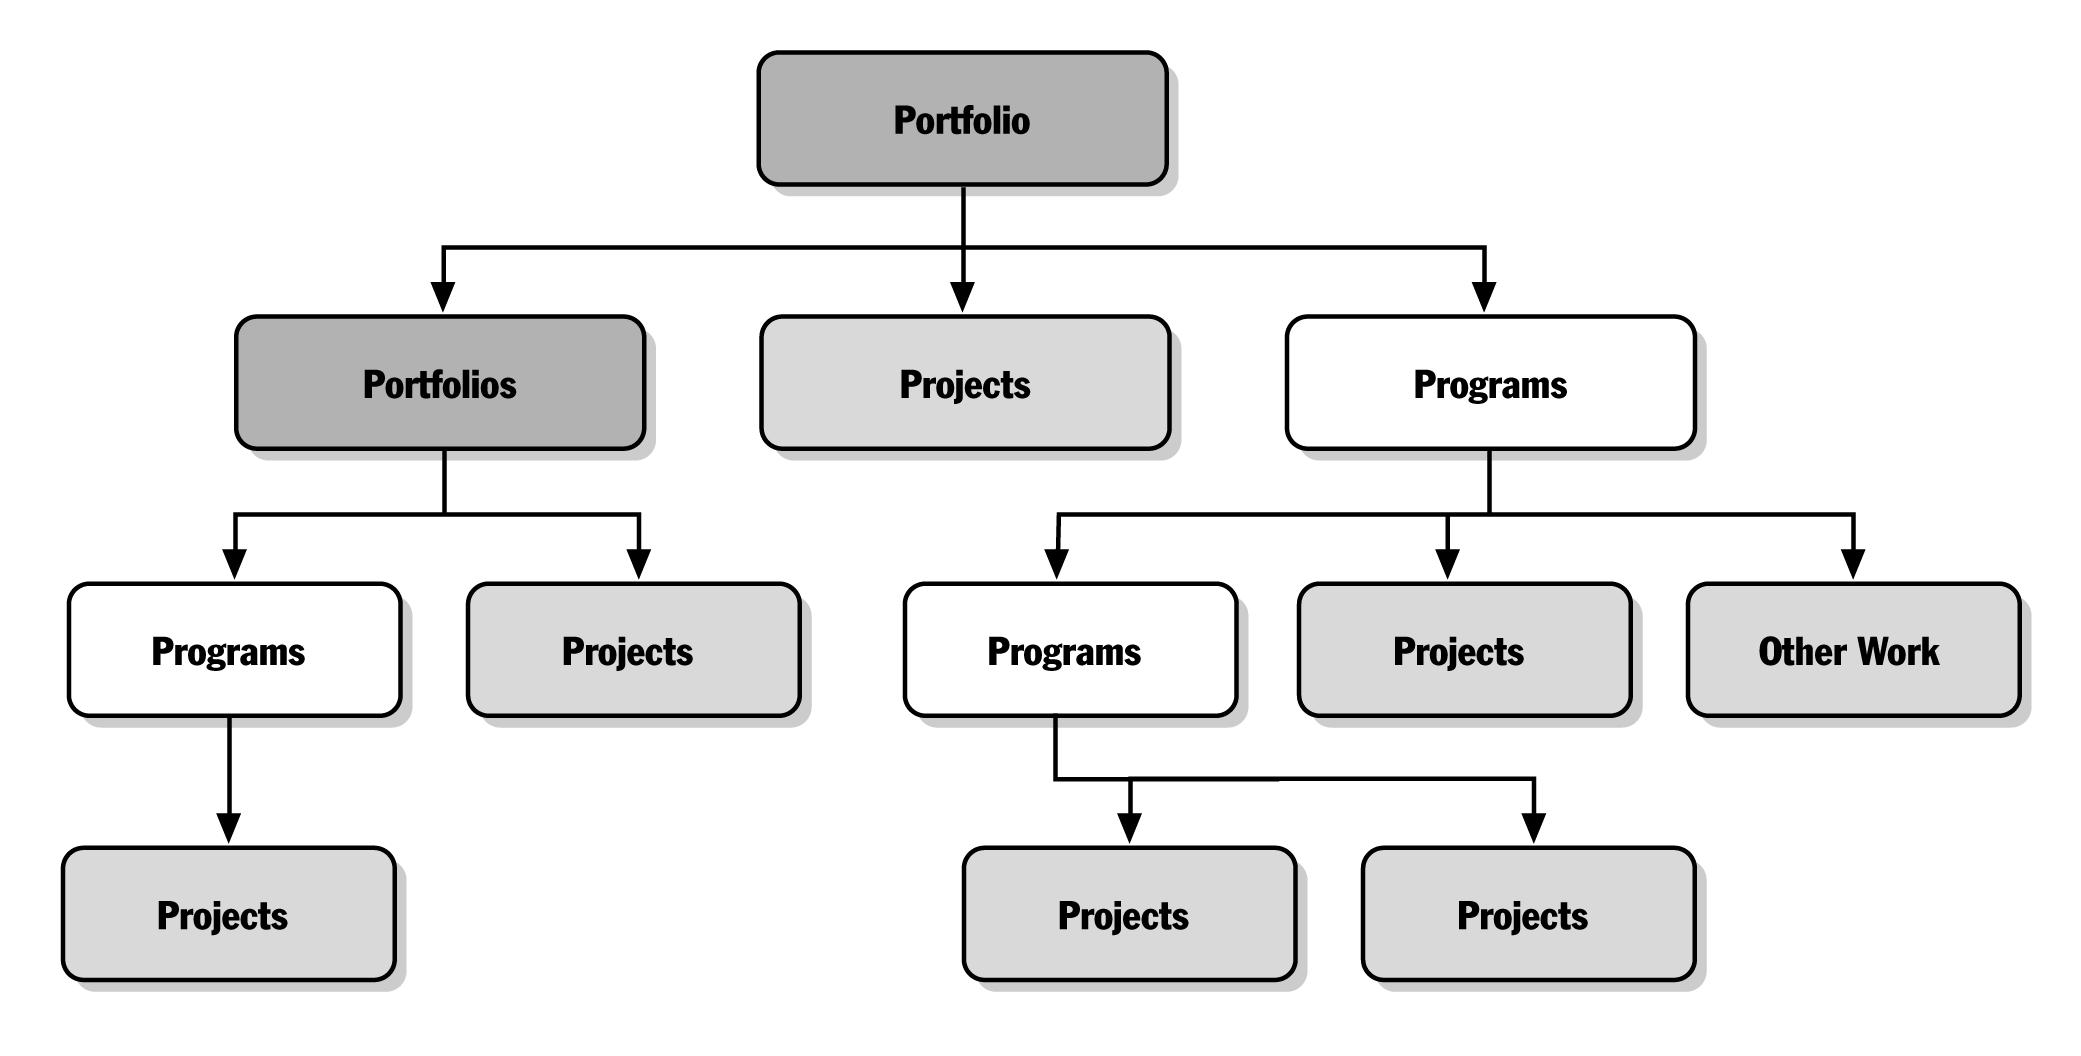
\includegraphics[width=.9\textwidth]{flow_sppm.jpg}
\caption{Exemplo dos relacionamentos de um Portfólio}
\end{figure} 

A Gerência de Portfólio de Projetos pode ser compreendida como a governança sobre o conjunto dos projetos. Ela atua em duas frentes: selecionando os 
projetos que devem ser executados; e, uma vez em execução, avaliando se estes projetos continuam viáveis e aderentes aos critérios pelos quais foram
aprovados.

O objetivo da etapa de seleção é criar uma combinação de projetos que melhor apóie os objetivos da organização, alinhada com as suas estratégias e 
com as restrições de recursos (pessoas e orçamento)(LEVINE, 2005).

Apesar de não estar completamente ciente deste fato, toda organização pratica algum tipo de gestão de portfolio em seus projetos. Projetos são aprovados 
quase que rotineiramente e/ou em momentos específicos dos ciclos de gestão das empresas. Gestão de projetos tornou-se, de fato, prática importante nos 
últimos anos com as organizações demandando profissionais certificados pelo PMI e alocação de recursos para estruturas especializadas de projeto, 
como Project Management Offices. 

Muitas empresas, no entanto, organizam seus projetos de forma ad-hoc e individualizada, com foco na determinação de prazos, realocação de recursos 
baseados em necessidades de curto prazo em constante mudança e soluções de disputas políticas sobre estes recursos escassos.\cite{artigo}

Porém muitas organizações necessitam de um gerenciamento que seja capaz de integrar seu vasto número de projetos aos objetivos estratégicos traçados.
Neste momento é que se faz necessária a utilização de uma gestão de portfolio, que será responsável por ajudar as empresas a gerenciarem o conjunto 
(projetos e estratégia) como um todo, de forma transparente e sistematizada. 

Para isso será necessária a utilização de métodos e práticas para priorizar e cancelar projetos, alocar recursos, definir responsabilidades, fazer o 
gerenciamento dos riscos e definir se será necessário o engajamento de terceiros, sem esquecer que tudo isso deverá ser feito levando em conta o 
planejamento estratégico definido pela organização.

Para que a gestão seja utilizada de forma otimizada a organização deverá possuir um gerenciamento de projetos consistente, de forma que seja possível 
levantar os dados relevantes para a gestão, tais como: tempo de desenvolvimento, recursos utilizadas, pessoal, investimento. Ou seja, para que a gestão 
de portfolio funcione a organização precisa também de uma gestão de conhecimento atuante.

Na tabela um são apresentados as etapas inerentes a gestão de portfolio e os respectivos detalhes de sua execução.

\begin{table}[H]
\begin{center}
 \begin{tabular}{| >{\centering\arraybackslash}m{2in} | >{\centering\arraybackslash}m{4in} |}
  \hline
  Passos & Detalhes \\
  \hline
  Identificação de projetos & Consideração dos aspectos estratégicos; \\
			    & Consideração dos aspectos táticos; \\
                            & Consideração dos projetos em andamento; \\
			    & Formar relação inicial de projetos. \\
  \hline
  Alinhamento de oportunidades às estratégias e à organização & Identificação e seleção  de critérios\\ 
							      & de avaliação estabelecendo pesos\\
							      & para avaliação dos projetos/programas;\\
							      & Hierarquização de projetos e programas.\\    
  \hline
  Avaliação de investimentos e recursos  & Pontos de decisão ou filtros levando-se\\
					 & em conta os elementos financeiros.\\
  \hline
  Desenvolvimento do portfolio & Formação do portfolio;\\ 
			       & O portfolio subsidiará decisões sobre\\
                               & projetos considerando-se priorização\\
			       & dos mesmos, possibilidades de exclusão,\\
                               & de inclusão de recursos, etc;\\
			       & O portfolio poderá também ser um\\
		               & instrumento para revisão do escopo dos projetos.\\
  \hline
  Gerenciamento do Portfolio   & Desenvolver estrturação dos projetos\\
			       & em termos de escopo, prazos e custos;\\
                               & Acompanhar o andamento;\\
                               & Liberar recursos;\\
                               & Comunicar os interessados, entre\\
			       & outras ações gerenciais.\\			      
  \hline			
 \end{tabular}
\caption{Processo gerencial para criação do gerenciamento de portfolio\cite{crawford}}
\end{center}
\end{table}

O conceito de projetos deverá estar bem definido, a forma como estes serão e são realizados, para que seja possível estimar o volume adequado de trabalho,
sem esquecer que estes sempre deverão estar atrelados a estratégia vigente e à disponibilidade de recursos. Além disso será necessário criar nos membros 
da organização a cultura de utilização dessas não tão novas metodologias, já que eles serão os responsáveis por fazer com que o processo como um todo 
funcione.

\section{Gestão de Portfólio e os processos organizacionais}
A gestão de portfolio deve combinar o foco da organização para garantir que os projetos selecionados atendam a estratégia de investimento do 
portfolio com o foco de gerenciamento de projetos na execução destes de forma eficaz e dentro da contribuição prevista para o portfolio.

A figura a seguir mostra as relações gerais entre os processos estratégicos e táticos da organização. A partir da visão e missão, a estratégia e 
objetivos organizacionais são desenvolvidos.

\begin{figure}[H]
\centering
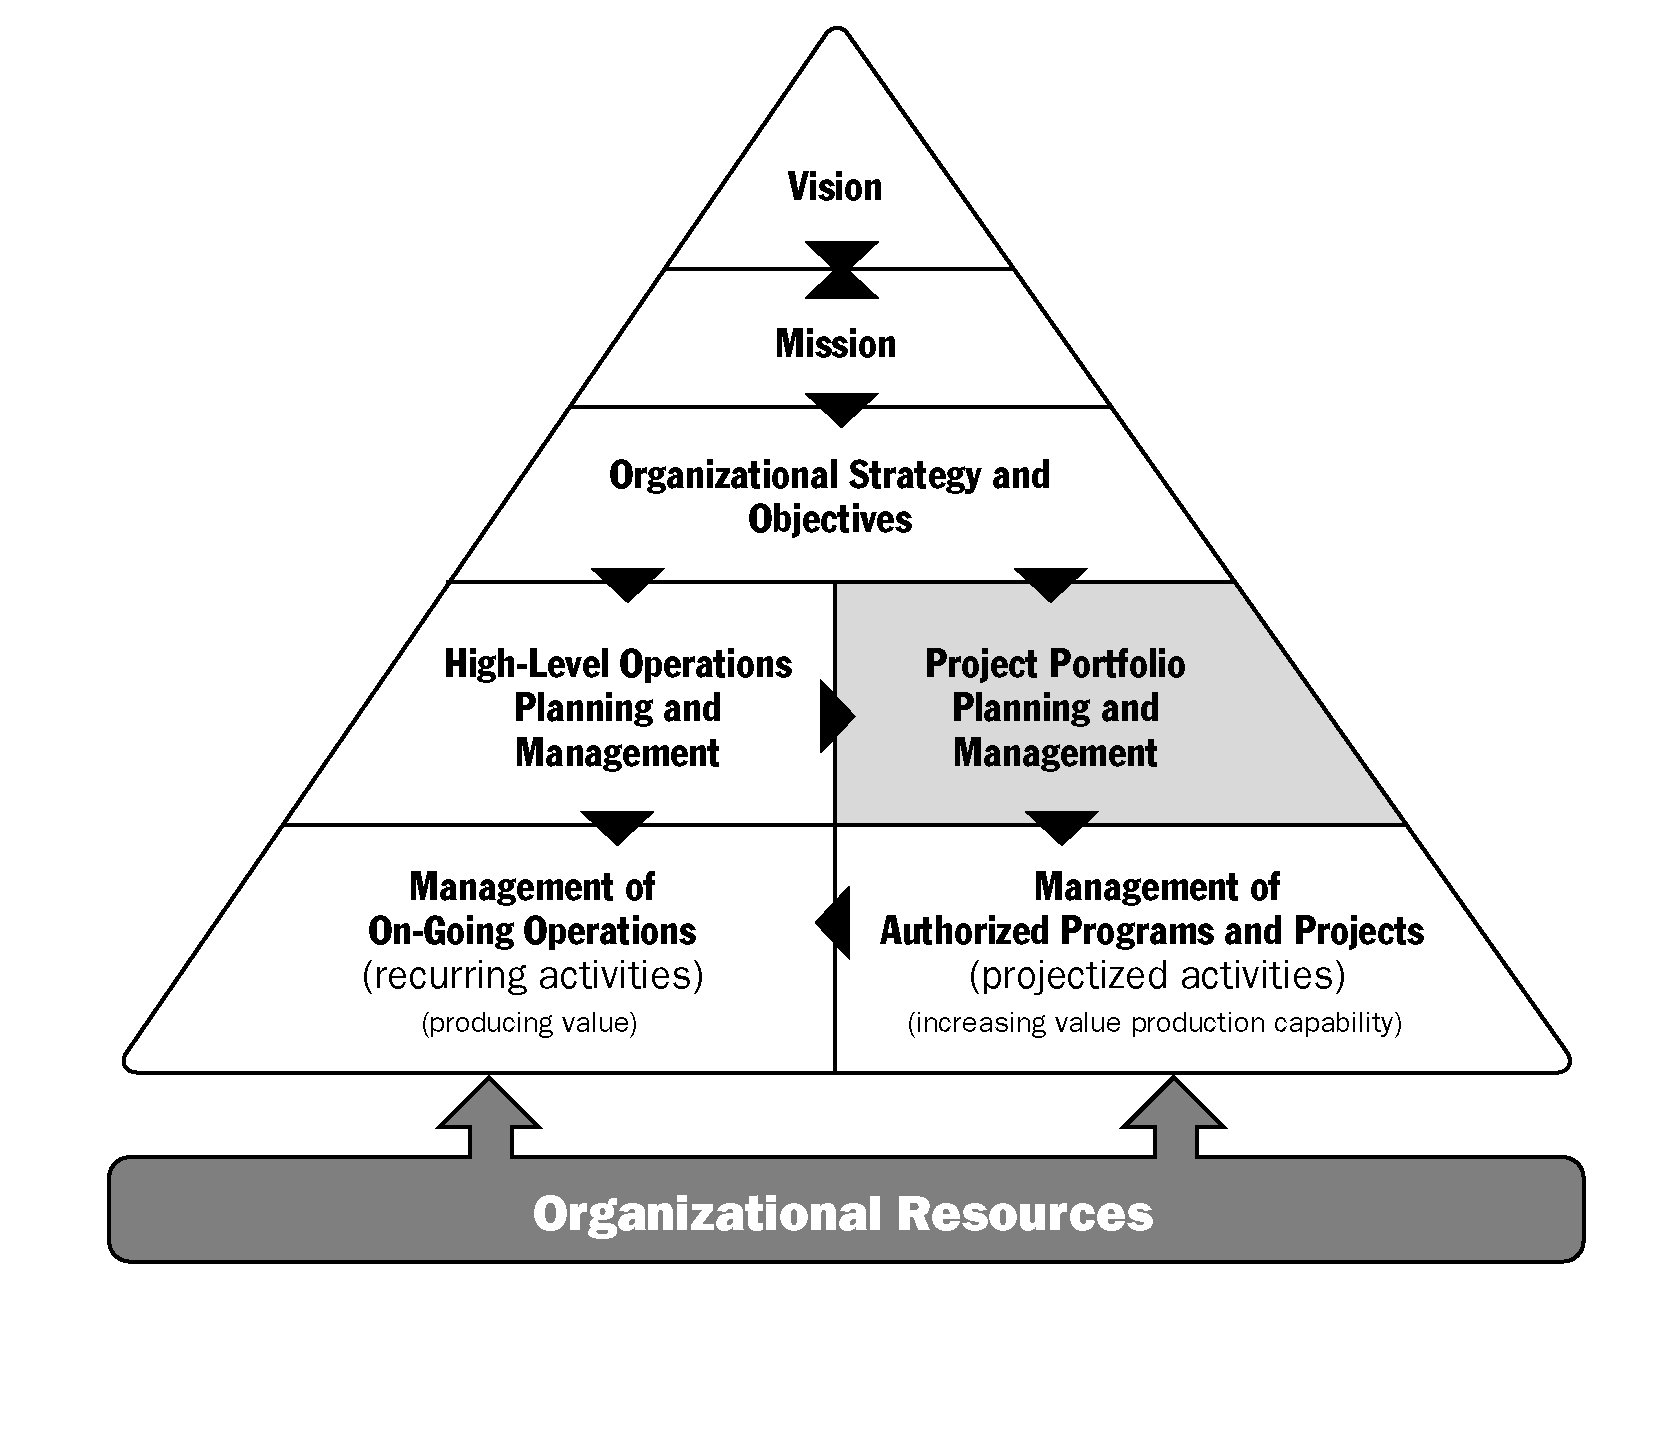
\includegraphics[width=.9\textwidth]{organizacional_port.jpg}
\caption{Contexto organizacional}
\end{figure}

A parte superior do triângulo (``Visão'', ``Missão'', ``Estratégia Organizacional e Objetivos'') ilustra os componentes utilizados para definir  as metas 
ou objetivos. Esses componentes são utilizados para direcionar todas as ações da organização. 

Observe que as setas na Figura 3 fornecem o contexto geral de influenciar as relações entre os elementos. Ou seja, o fluxo das ações, podemos verificar que mesmo as ações que ocorrem no mesmo nível, como é caso 
das Operações de alto nível e o gerenciamento de portfolio acabam por influenciar um ao outro.

O meio do triângulo (``Planejamento e Gestão de operações de alto nível'' e ``Planejamento e gestão do portfolio de projeto'') representa os processos 
que estabelecem ações adequadas para atingir as metas. Esses processos interagem com a parte inferior do triângulo, em que a contribuição de todas as 
atividades operacionais deve ser comparada à criação de valor em curso. E a contribuição de todas as atividades do projeto devem ser comparados com a 
criação do novo valor.

``Gestão de operações em curso'' e ``Gestão de Programas e Projetos Autorizados'', que aparecem na parte inferior do triângulo, correspondem aos 
componentes que garantem as operações da organização e que os portfolios sejam executados de forma eficaz e eficiente.\cite{sppm}

Ambos os aspectos operacionais e de projeto de uma organização devem ser considerados na gestão de portfolio. O lado operacional da organização, faz 
uso recorrente de atividades e processos de operações de gestão que facilitam o planejamento efetivo do nível elevado. 

Já pelo lado dos projetos da organização temos a utilização de programas/processos de gerenciamento de projetos que permitem o planejamento eficiente do 
projeto e as atividades de implementação.

Ao nível da gestão táctica, a pergunta é: ``Esta operação ou projeto está sendo gerenciado de forma eficiente com melhores resultados, com uma utilização 
ótima dos recursos, com o esforço ótimo, e em conformidade com os valores organizacionais e normas?''

A aplicação de gestão de portfolio, como citamos no início deste capítulo, deve permitir a interligação dos objetivos organizacionais com as estratégias de 
gerência através do compartilhamento de objetivos e a alocação de recursos. O fluxo de controle é a seguinte: \cite{sppm}

\begin{itemize}
 \item Propósito estratégico e a priorização de orientar para a determinação dos recursos financeiros que devem 
ser atribuídos ao portfolio.
  \item A intenção estratégica é mapeada em um conjunto de componentes do portfolio (ou seja, projetos e programas), inclusive na alocação 
dos recursos. Esses componentes são gerenciados de acordo com os princípios de gestão do portfolio descritos na ``Standard of Portfolio Management''.
  \item Cada programa corresponde ao subconjunto delegado da intenção estratégica global, que irá disponibiliza-los por meio dos recursos alocados.
  \item Cada projeto é definido pela sua contribuição à intenção estratégica do portfolio, e
pode ser gerenciada de acordo com os princípios do PMBOK e outros princípios, conforme apropriado.
\end{itemize}

Neste sentido, o portfolio funciona como um elo entre a visão e os objetivos que constam da estratégia organizacional e a execução de atividades que 
levarão ao cumprimento dos objetivos. A estratégia organizacional dá o direcionamento para a priorização e distribuição de recursos entre os componentes. 
Por outro lado, o portfolio deve refletir esta estratégia e cada componente deve ser responsável por um subconjunto de objetivos estratégicos a serem 
atingidos.\cite{ricardo}

Há que se considerar que no contexto da gestão de portfolio, o vínculo dos projetos com a estratégia da empresa pode ser realizado por meio de duas 
abordagens. A primeira é top-down, utilizando a visão, metas e planos estratégicos da organização para um plano de ataque com definição de prioridades 
de alocação de recursos para programas e projetos. A outra é bottom-up: indutivo e distribuído na organização por meio da proposição individual de 
projetos: indicadores de alinhamento na avaliação individual dos projetos. 

É importante ressaltar que as duas abordagens são complementares, uma compensa as limitações da outra e que uma boa gestão de portfolio precisa ser 
capaz de contemplar ambas as situações.\cite{artigo}

\section{Selecionando projetos}
Um dos maiores desafios da gestão de portfolio é selecionar os projetos corretos, fazendo com que esses tenham maior prioridade. Existem diversas 
técnicas para seleção dos projetos, aquelas que levam em conta a demanda de recursos e esforços que determinado projeto necessitará, os riscos envolvidos,
custos, tempo e outros. 

A definição de uma metodologia para a seleção de projetos é um processo estratégico que deve ser feito antecipadamente a outros processos relacionados à 
seleção, a fim de proporcionar o alinhamento estratégico dos projetos. Tal metodologia deve ser flexível, baseada no entendimento dos tomadores de 
decisão a respeito das formas de selecionar existentes e na disposição para aprender novas abordagens\cite{archer}.

De acordo com Carl Neun, o CFO da Wilsnville \cite{johnson}, “A realidade é que quando alocamos grandes investimentos, técnicas fazem uma grande 
diferença”. Os tomadores de decisão da organização necessitam de critérios que sejam dinâmicos porém consistentes para avaliar as oportunidades e selecionar
o conjunto de projetos capazes de refletir os objetivos estratégicos traçados. Sendo assim, podemos dizer que a gestão do portfolio é o caminho.

O planejamento estratégico deve ser capaz de balancear os esforços da organização em termos de prazos curtos versus prazos longos, crescimento versus retorno
monetário, ciclo de vida do negócio, oportunidades de mercados, entre outras, tudo isso sem esquecer que a organização deverá manter uma saudável gestão
de riscos.

Vamos apresentar agora algumas técnicas e frameworks criados para o auxílio dessa primeira etapa da gestão, lembrando que se os projetos selecionados 
estiverem em desacordo com as metas organizacionais há grande possibilidade da gestão de portfolio se tornar ineficaz ou insatisfatória.

\subsection{Método dos Fatores Críticos de Sucesso}
Uma das primeiras propostas para o problema de seleção e priorização de projetos de TI foi o método dos Fatores Críticos de Sucesso (FCS),
proposto por \cite{rockart} . Esse método, que ainda é amplamente utilizado, foca, principalmente, os sistemas de informação gerenciais
e executivos, e é baseado na definição, por parte dos altos executivos, das atuais necessidades representadas pelos FCS.

Ainda segundo\cite{rockart} os FCS podem ser definidos como as áreas onde um resultado sendo satisfatório ``garante o sucesso competitivo da organização",
e define também que os principais FCS poderão ser identificados em diversos setores, tais como a estrutura de um setor em si, na posição da indústria, 
na localização geográfica e nos fatores ambientais e temporais.

Faz-se necessário destacar também a importância do posicionamento da empresa em sua indústria, de forma a obter vantagens competitivas sunstentáveis por 
meio da escolha de uma das três possíveis estratégias genéricas: liderança em custos, diferenciação e foco.  

A competitividade de uma indústria resulta da ação de cinco forças: clientes, fornecedores, produtos substitutos, novos entrantes e a rivalidade entre 
os competidores atuais. Quanto mais intensas forem essas forças, maior a concorrência entre as empresas de uma indústria e, por conseguinte, menor o 
potencial de lucratividade.\cite{porter1, porter2} 

\subsection{Grid Estratégico}
Uma outra importante análise da seleção de projetos foi realizada por \cite{mcfarlan}, essa seleção é feita levando em consideração os riscos associados
a cada projeto e também os riscos do portfolio como um todo. Onde esses riscos incluem custo, prazo, desempenho técnico, superstimação dos benefícios 
dos sistemas e incompatibilidade de hardware e/ou software com o sistema. 

O Grid Estratégico, uma técnica que permite a visualização da relação entre a estratégia de TI, atual e a carteira de aplicações (futuro), foi proposta 
por \cite{mcfarlan} e define quatro regiões, cada qual representando um possível papel para a TI dentro da organização, são elas: Suporte, Fábrica, 
Tranformação e Estratégico.

\begin{figure}[H]
\centering
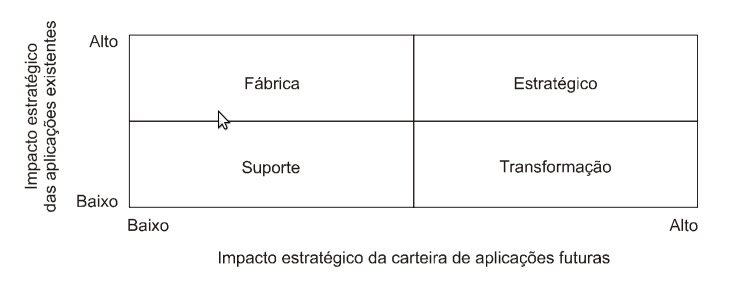
\includegraphics[width=.9\textwidth]{grid_estrategico.jpg}
\caption{Grid Estratégico do impacto das aplicações de TI\cite{mcfarlan}.}
\end{figure} 

\begin{itemize}
 \item Suporte: as aplicações presentes e futuras de TI têm pouca influência na estratégia da
	organização.
  \item Fábrica: as aplicações da TI são importantes para o sucesso da operação da empresa, 
	mas não há nenhuma aplicação estratégica planejada para o futuro.
  \item Transformação: a TI está saindo de uma situação de baixa importância (região de
	Suporte) para assumir um papel de importância estratégica na organização, em
        face das novas aplicações de TI planejadas para ser implementadas no futuro próximo.
  \item Estratégico: a TI é muito importante na estratégia atual do negócio e as novas apli-
        cações planejadas manterão a importância estratégica da TI no futuro.
\end{itemize}

\subsection{Modelos de Pontuação}
Os modelos de pontuação são um método numérico, onde é permitido levar em consideração diversos critérios quando se faz a comparação dos projetos. Cada
critério deverá ser avaliado em uma escala de 1-5 ou 0-10, após tal avaliação os pontos serão multiplicados por pesos somados. A partir disso é possível
obter uma pontuação individual para cada projeto. 

Ao utilizar um modelo de pontuação, a seleção dos critérios deverá ser feita de forma cuidadosa e o refinamento dos critérios poderá levar anos. No modelo 
de pontuação desenvolvido por Hoechst, são apresentados critérios que foram selecionados cuidadosamente e expressos em palavras, além de terem sido definidos 
operacionalmente, foram testados e validados em busca de consistência por anos. Grande parte dos fatores utilizados por Hoechst encontra-se na tabela dois.

\begin{table}[H]
\begin{center}
 \begin{tabular}{| >{\arraybackslash}m{6in} |}
  \hline
  Retorno (para a companhia) \\
  \ \ \ \ \ \ \ Absoluta contribuição para rentabilidade da empresa\\
  \ \ \ \ \ \ \ Retorno tecnológico\\
  \ \ \ \ \ \ \ Tempo para o início da comercialização\\
  \hline			
  Alinhamento à estratégia do negócio \\
  \ \ \ \ \ \ \  Congruência (quão alinhado o projeto está em relação à estratégia da companhia)\\
  \ \ \ \ \ \ \ Impacto (financeiro e estratégico do produto sobre o negócio da companhia)\\
  \hline			
  Influência estratégica (habilidade do projeto de alavancar recursos da companhia) \\
  \ \ \ \ \ \ \ Posição proprietária\\
  \ \ \ \ \ \ \ Crescimento da plataforma\\
  \ \ \ \ \ \ \ Durabilidade\\
  \ \ \ \ \ \ \ Sinergia\\
  \hline			
  Probabilidade do sucesso comercial\\
  \ \ \ \ \ \ \ Existência da necessidade de mercado\\
  \ \ \ \ \ \ \ Maturidade do mercado\\
  \ \ \ \ \ \ \ Intensidade competitiva\\
  \ \ \ \ \ \ \ Existência de desenvolvimento de aplicação comercial\\
  \ \ \ \ \ \ \ Suposições comerciais\\
  \ \ \ \ \ \ \ Impacto regulatório, social e político\\
  \hline			
  Probabilidade do sucesso técnico\\
  \ \ \ \ \ \ \ Gap técnico\\
  \ \ \ \ \ \ \ Complexidade do projeto\\
  \ \ \ \ \ \ \ Existência das habilidade tecnológicas\\
  \ \ \ \ \ \ \ Disponibilidade de pessoas e facilidades\\
  \hline			
 \end{tabular}
\caption{Critérios de classificação de projetos usados por Hoechst\cite{cooper}}
\end{center}
\end{table}

São apresentados cinco fatores principais: retorno, crescimento estratégico, alinhamento estratégico, probabilidade de sucesso técnico e probabilidade de
sucesso comercial. Estes são divididos em critérios menores, sendo dezenove ao total. Cada um destes será pontuado pela gerência, podendo variar de 0 a 10.

Os pontos de cada fator serão encontrados a partir do cálculo da média dos critérios de cada fator. Sendo assim, a pontuação final do projeto poderá ser 
encontrada pela soma da pontuação de todos os fatores. Essa pontuação será utilizada na priorização e tomada de decisões do tipo ``Go and Kill''.

\subsection{Diagrama de Bolhas}
Diagramas de bolhas é um método bastante conhecido e eficiente de suporte a decisões que dizem respeito a seleção e priorização de projetos. Com tais
digramas, será possível apresentar em formato visual a composição completa de um portfolio, fornecendo assim uma melhor percepção do balanceamento do
portfolio. \cite{cooper2}

Através de um plano bidimensional, onde é possível visualizar os eixos X e Y, mostram-se os projetos de um portfolio. E poderemos determinar que os 
valores de X e Y sejam pertencentes a qualquer dimensão de interesse, como por exemplo: risco, retorno, tempo, etc., porém algumas dimensões já se 
tornaram padrões, tais como Risco x Retorno.\cite{cooper}

Outra possibilidade na utilização do diagrama de bolhas, é torna-lo mais rico através da utilização de novas cores, tamanhos e preenchimento dos círculos.
Onde cada uma dessas características denotem um fato importante inerente ao projeto a ser avaliado.

A figura A SEGUIR apresenta um diagrama de bolhas, onde o tamanho diz respeito a quantidade de recursos que será necessária para o desenvolvimento do projeto
e o preenchimento representa o tipo de projeto.

\begin{figure}[H]
\centering
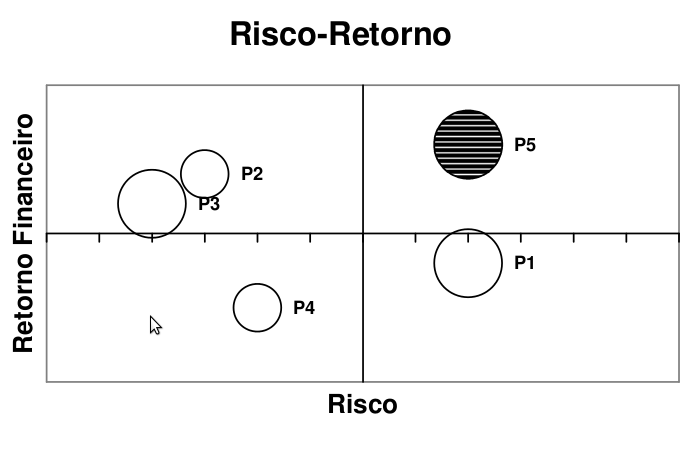
\includegraphics[width=.9\textwidth]{diagrama_bolhas.png}
\caption{Exemplo diagrama de bolhas\cite{cooper}.}
\end{figure} 

\subsection{Modelo de Archer para seleção}
Com o intuito de simplificar o processo para a seleção de projetos \cite{archer} propõe um modelo para gestão de portfolio, esse modelo utiliza a 
segmentação do processo em fases e estágios, desde as considerações referentes à estratégia inicial (que é a etapa mais ampla) até a montagem final do 
portfolio.

A figura a seguir apresenta o fluxo do modelo, onde é possível observar quais são as etapas primordiais para a seleção dos projetos que deverão comportar
o portfolio.

\begin{figure}[H]
\centering
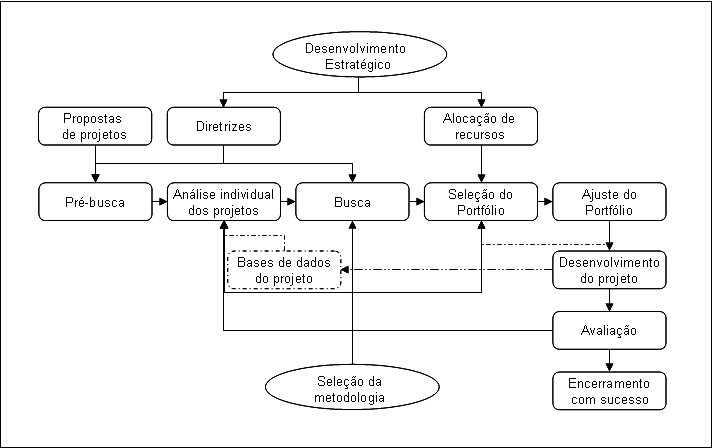
\includegraphics[width=.9\textwidth]{archer.jpg}
\caption{Framework para a seleção de projetos no portfolio\cite{archer}.}
\end{figure}

O modelo apresentado pode ser dividido basicamente em três etapas: pré-processo, processo de seleção (possui fases) e pós-processo. As características 
de cada estágio estão representadas no quadro a seguir e envolvem opções de metodologias ou ferramentas para a sua realização, a fim de obter a máxima 
cooperação dos tomadores de decisão durante o processo de seleção dos projetos no portfolio \cite{archer}. 

\begin{table}[H]
\begin{center}
 \begin{tabular}{| >{\arraybackslash\small}m{1.4in} | >{\arraybackslash\small}m{1.3in} | >{\arraybackslash\small}m{1.1in} | >{\arraybackslash\small}m{2in} |}
  \hline
  \rowcolor{purple} Estágio do processo & Estágio de seleção & Atividades & Metodologias potenciais \\
  \hline
   Pré-processo & Desenvolvimento da estratégia & Mapa estratégico, matriz de portfolio & Definidas na estratégia da organização \\
  \hline
  Processo de seleção do portfolio & Pré-busca & Rejeição de projetos que não atendam aos critérios & Critérios, foco estratégico, estudos de viabilidade \\
  \hline
	  &  & & \\
  \hline
 \end{tabular}
\caption{Critérios de classificação de projetos usados por Hoechst\cite{cooper}}
\end{center}
\end{table}

\begin{figure}[H]
\centering
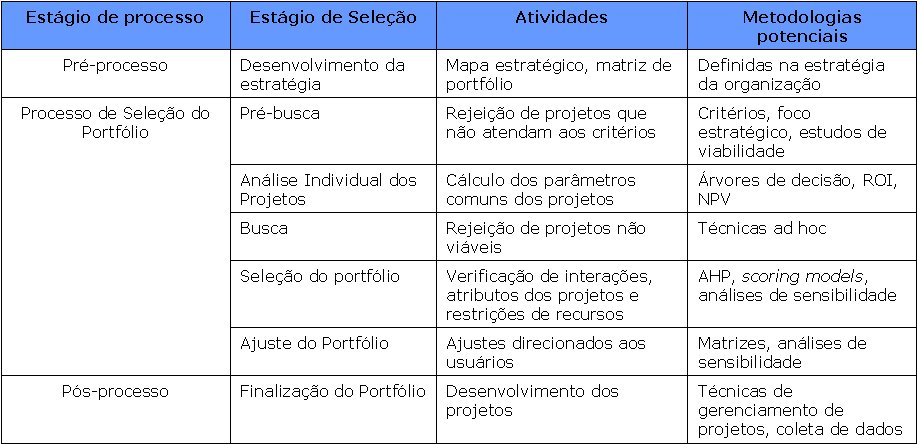
\includegraphics[width=.9\textwidth]{tabela_archer.jpg}
\caption{Atividades e metodologias no framework de seleção do portfolio\cite{archer}.}
\end{figure}

\section{Benefícios da Gestão de Portfólio}
Existem diversos benefícios em se utilizar a gestão de portfolio, como já citado, a mesma provê uma visão mais ampla de todos os projetos da instituição 
e a situação em que estes se encontram.

A ferramenta utilizada para o controle da gestão pode ainda trazer outras informações que também necessitam ser avaliadas pelos altos executivos da 
organização nas tomadas de decisão quanto a manter ou não um projeto e ainda as prioridades referentes a escolha.

Entre os principais benefícios da gestão de portfolio podemos citar:\cite{atila}

\begin{itemize}
 \item Eliminação de projetos duplicados. Projetos idênticos, ou muito similares, sendo conduzidos em duas ou mais áreas na empresa podem ser fundidos em um só, reduzindo custos e evitando incompatibilidades no futuro.
 \item Combinação de projetos gerando economias de escala. Projetos que, embora não sejam idênticos, fazem sentido de serem executados juntos, pela mesma equipe e próximos no tempo. Um exemplo seriam projetos que produzem muitas entradas um para o outro.
 \item Visão clara da interdependência entre projetos. É mais fácil perceber quais saídas do projeto A devem ser entradas para o projeto B e vice-versa.
 \item Orienta a coordenação no tempo de diferentes projetos: o que deve acontecer no projeto A antes que se possa executar a tarefa X no projeto B.
 \item Redução da prioridade de projetos necessários, mas menos importantes ou urgentes. Ao comparar o escopo do projeto com as necessidades estratégicas da organização, é possível detectar quais projetos podem ser deixados para depois, quando houver mais recursos disponíveis.
 \item Aumento da prioridade de projetos estratégicos, mas de baixa visibilidade. Da mesma forma, o exame da relevância do projeto para o cumprimento das metas estratégicas pode levar à priorização e alocação de recursos adicionais a um projeto cuja visibilidade esteja baixa, 
talvez por falta de patrocinadores poderosos.
 \item Otimização da alocação de recursos e talentos. A Gestão de Portfolio de Projetos provê orientação na formação de equipes, usando as habilidades das pessoas onde contam mais. Se existe alguém na organização que é um expert em uma das fases-padrão dos projetos normalmente 
executados, por que esta pessoa deveria estar “fixa” em uma equipe que pega um projeto após o outro, participando também das atividades nas quais não é tão bom assim? Se João é um ótimo especificador de requisitos, mas um desenvolvedor apenas mediano, que sentido tem ele fazer 
tudo na equipe? Não é melhor que ele especifique os requisitos no projeto A, depois vá fazer o mesmo no projeto B e assim por diante? Com a visão global que a Gestão de Portfolio dá, é possível planejar melhor o emprego dos especialistas nos diversos projetos.
 \item Visão clara do que deve ser feito pela “prata-da-casa” e o que pode ou deve ser terceirizado. Projetos críticos que exijam a participação intensa de pessoal interno são mais facilmente identificados, de modo que podemos deixar os outros projetos como candidatos à terceirização.
 \item Identificação de necessidades de contratação e treinamento. Como a Gestão de Portfolio provê uma visão de médio a longo prazo para os projetos da organização, é possível identificar com bastante antecedência quais serão as competências necessárias no momento em que os projetos 
começarem. Nada de treinar pessoas depois que o projeto já começou! Da mesma forma, é possível antecipar se será necessário trazer gente nova para o time.
\end{itemize}

\section{Desafios da Gestão de Portfólio}
Apesar de ser aparentemente simples integrar os projetos e processos da organização as metas estratégicas traçadas, a gestão de portfolio encontra alguns 
desafios. Sendo o principal deles a priorização dos projetos. A forma como será definido para que projeto determinados recursos deverão ser alocados, 
levando em conta a existência de recursos escassos, ou seja, como dividir tais recursos entre os projetos existentes.

Segundo Cooper (2001), as principais causas para um fraco gerenciamento de portfolio são:
\begin{itemize}
 \item Estratégica;
 \item Projetos de baixo valor;
 \item Falta de foco;
 \item Projetos errados.
\end{itemize}

Visto que os recursos são escassos, as principais questões são: a priorização de projetos e a realocação dos recursos. Sendo assim, há uma forte competição 
por recursos entre os projetos, e muitas vezes uma falta de clareza na prioridade dos projetos dificulta o gerenciamento do portfolio.

Outro grande desafio encontrado diz respeito a tomada de decisão sobre os investimentos, levando em consideração novamente a escassez de recursos e as 
necessidades estratégicas da organização. 

Ainda podemos colocar o balanceamento do portfolio como desafio final, ou seja, uma metodologia que consiga 
desenvolver uma prática balanceada para a escolha do investimento ideal entre o risco do portfolio e o retorno, a manutenção necessária e o crescimento 
alcançado, projetos curtos e projetos longos.\cite{cooper}

\chapter{Modelos para Gestão de Portfólio} 
A elaboração de um modelo deve levar em conta os principais desafios apresentados para a questão e uma solução para tais. Caso essas questões não sejam 
observadas e estudadas, o modelo proposto poderá pender para um ou outro benefício da gestão, o que não resolverá o problema como um todo e será apenas 
mais  uma alternativa e não uma solução de fato. 

Para que seja possível elaborar um modelo deve-se também levar em conta os problemas específicos identificados na literatura teórica referente ao
gerenciamento de portfolio, ou seja: falta de alinhamento estratégico; baixa qualidade da carteira; faltas de critérios formais; interdependência 
técnica/comercial, entre outros \cite{martino1, martino2, cooper}.

A seguir serão apresentados alguns dos modelos estudados, suas definições e detalhes pertinentes para seu entendimento.

\section{Cooper, Edgett e Kleinschmidt}
Para Cooper a gestão de portfolio pode ser definida por dois processos chaves, sendo eles: ``Stage and Gate'', onde são realizadas as tomadas de 
decisões individuais sobre cada projeto; e o ``Go and Kill``, onde são realizadas as revisões de projetos individuais em andamento e revisões 
sobre o portfolio que vem sendo trabalho. Nesta seção apresentaremos mais detalhes sobre tais processos.

Em Cooper et al, o processo de gestão de portfolio é descrito como um sistema integrado de tomada de decisão, sendo que a condição básica para tal definição
é ``que a escolha de projetos de novos produtos é a operacionalização da estratégia''. Dessa forma, é possível verificar que o autor considera que a definição
da estratégia de negócios é responsável por influenciar grande parte das etapas existentes em seu modelo.

A primeira etapa do modelo, ``Stage and Gate'', é um processo formal utilizado pelas organizações para que seja possível efetuar a segunda etapa, o processo
``Go and Kill'' sobre projetos individuais. Como observamos em capítulos anteriores, projetos tem como definição alguns estágios (Ex.: idealização, planejamento,
execução,...). 

Após cada estágio, um projeto passara por um processo de decisão, nomeado passagem (``Gate''), que consiste na avaliação por um grupo de gerentes se este 
deverá continuar ou finalizar ( ``Go and Kill''), nessa etapa é também possível tomar decisões relacionadas a priorização do projeto em questão. Além disso
nas passagens é o momento de realizar a alocação de recursos necessários para o desenvolvimento do mesmo.

Deve-se lembrar que os critérios utilizados para avaliação realizada nos ``Gates'' devem ser bastante consistentes e levar em consideração as metas e objetivos
traçados estrategicamente pela organização, pois nessa etapa, projetos que não serão capazes de alcançar tais parâmetros serão eliminados. Levando em conta
que vários critérios são frequentemente requeridos para selecionar projetos, é recomendável a utilização de um modelo de pontuação (scoring model) nesta etapa.

Os modelos de pontuação tem sido adaptados e modificados ao longo dos anos, e por passarem por tais processos sua utilização é apontada como imprescindível 
na etapa de seleção de projetos e também no momento de definir aqueles que terão continuidade. 

Tais modelos podem ser utilizados na construção dos objetivos traçados pela organização no momento do planejamento estratégico, onde teremos metas e 
critérios já determinados, e também com suas prioridades bem definidas.

A segunda etapa do projeto leva em consideração a pontuação final recebida pelo projeto no processo anterior. Essa pontuação poderá ser realizada durante o
``Gate'' ou ainda previamente pelos responsáveis da área em questão. 

Os recursos serão alocados nos projetos aprovados neste momento (go projects), e em seguida será realizado um processo de priorização relativa dos 
projetos (levando em conta a pré-alocação dos recursos realizada na etapa anterior) com base na pontuação individual recebida.

Mesmo sendo possível afirmar que a classificação dos projetos realizada utilizando-se critérios financeiros somados a outros, os modelos de pontuação
apresentam falhas com frequência quando asseguram que os portfolios estão completamente alinhados com a estratégia organizacional e balanceados de forma ótima.

A pontuação é capaz de maximizar lucros e pontuação de um projeto em particular, mas também é capz de produzir uma lista de projetos desbalanceada ou apresentar
falha ao replicar os critérios organizacionais estabelecidos.

Assim, o alinhamento estratégico e o balanceamento do portfolio poderão ser alcançados através da construção de uma extensão dos critérios estratégicos ou
uma discussão do impacto gerado pelas decisões sob tais projetos individualmente no portfolio geral da organização. 

Podemos ainda utilizar modelos de pontuação que fazem uso de critérios estratégicos para alcançar tal alinhamento. Não esquecendo que fatores como riscos,
incertezas e probabilidade de sucesso devem ser levados em consideração no momento da tomada de decisão final sobre qual será o portfolio, e estes 
deverão ser visíveis e relembrados durante o processo de avaliação.

O processo de seleção de projetos também deverá ser capaz de lidar com mudanças e interações das metas da organização. Fazendo assim com que o sistema seja 
flexível e adaptável a realidade das metas, requisitos e características do projeto, que poderão sofrer alterações ao longo do tempo.A Figura a seguir 
apresenta a primeira etapa do modelo, ``Stage and Gate''.

\begin{figure}[H]
\centering
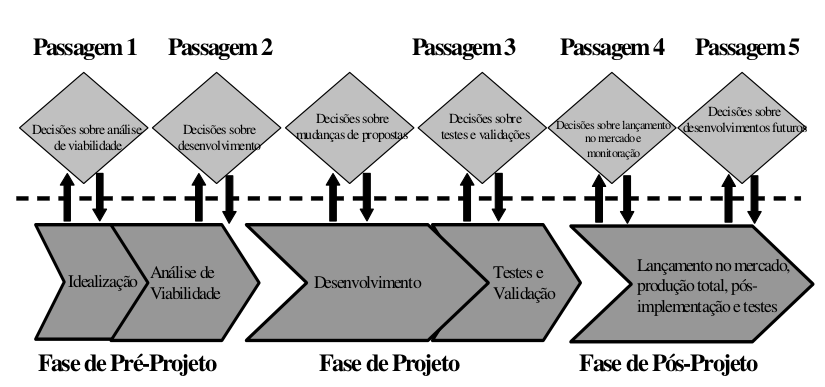
\includegraphics[width=.9\textwidth]{stage_and_gate.png}
\caption{Processo Stage and Gate}
\end{figure}

O modelo prevê também etapas de revisão do portfolio, que consistem basicamente em realizar uma reavaliação periódica do portfolio, que poderá ser feita
anualmente, semestralmente ou trimestralmente, ficando a critério da organização tal decisão. Nesta etapa, os projetos ativos passarão por uma revisão
e serão comparados aos demais, o balanceamento do portfolio será considerado sobre diversas dimensões. 

Essa é uma oportunidade de se obter uma visão holística e realizar considerações sobre todos os projetos existentes no momento. Poderão ser utilizadas 
diferentes ferramentas para um melhor aproveitamento desta etapa, dentre elas podemos citar: diagramas, gráficos, modelos financeiros e abordagens 
estratégicas.

Através destes é possível obter uma visualização mais claras das informações pertinentes ao portfolio e aos projetos individualmente, 
porém não serão fatores ou ferramentas utilizados para a tomada de decisão, será responsabilidade dos gestores definir quais projetos continuam e quais 
deverão ser finalizados.

Esta etapa tem como intuito verificar se a combinação ou balanceamento dos projetos está correta e gerando os resultados esperados. Deverá ser capaz de
identificar quais são as estratégias imperativas e os projetos imprescindíveis para atingi-las, bem como checar as prioridades dos projetos e fornecer uma
lista destes com suas pontuações e priorizações. 

Checar o alinhamento estratégico e o balanceamento do portfolio e realizar ajustes no modelo utilizado na etapa ``Gates''. Se todos os resultados 
encontrados estiverem de acordo com as expectativas e metas traçadas, tal etapa será utilizada apenas para correção de possíveis erros. 

A revisão do portfolio também deverá ser capaz de assegurar que as metas principais da gestão estão sendo respeitadas, lembrando que 
essas são: o máximo valor do negócio, balanceamento e ligação com a estratégia da organização.

A saída da etapa de revisão do portfolio pode gerar diferentes decisões, dentre elas a opção de ``matar'' alguns projetos ou definir nova prioridade, o que
como vimos, acontece também na etapa de passagem. Além dessas questões, aqui é possível também determinar e modificar os critérios e metas traçados inicialmente
para o portfolio, fazendo assim com que possa ser avaliada a efetividade e quem sabe a necessidade de se trabalhar o balanceamento dos projetos.

Dada as explanações apresentadas, é possível verificar que as etapas de passagens e revisão acabam por se sobrepôr, porém ambas possuem papel
importante na gestão do portfolio. A figura A SEGUIR demonstra as tarefas realizadas em cada uma das etapas.

\begin{figure}[H]
\centering
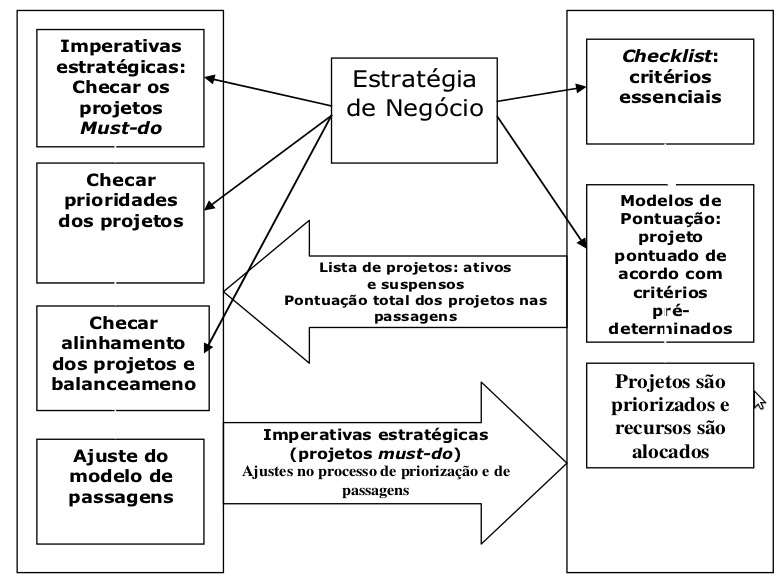
\includegraphics[width=.9\textwidth]{gpp_total_cooper.png}
\caption{Processos da Gestão de Portfólio\cite{cooper}}
\end{figure}

Cada projeto recebe atenção individual durante as decisões de passagem, ou seja, cada projeto irá mudar de um estágio para o outro de forma individual,
e terão suas características avaliadas de acordo com cada critério estabelecido individualmente ao longo do processo de passagem. 

Dessa forma, verificamos que os critérios e decisões são pensados e planejados levando em conta um projeto particular, mas se faz necessário considerar
a relação que existirá nas etapas seguintes com os demais projetos da organização.

O fator que pode ser apontado como diferencial entre as etapas de passagem e revisão, é que a segunda ocorre com datas pré-determinadas e deve levar em 
consideração o portfolio como um todo, além dos projetos individuais. 

Já a primeira diz respeito apenas ao projeto, e assim a discussão de critérios acaba por ser feita de forma mais particular. Enquanto a revisão deve 
levar em conta o balanceamento e o alinhamento estratégico ideal do portfolio final.

Sendo assim, pode-se verificar que o modelo em questão possui dois grandes blocos, a etapa ``Stage and Gate'' e a etapa de Revisão do Portfólio, sendo que
estes se comunicam entre si. O primeiro tem como intuito detalhar quais serão os critérios e os pontos de decisão, ou seja, os ``Gates'' propriamente ditos,
é possível detalhar essa etapa da seguinte forma:

\begin{itemize}
 \item Verificação do atendimento aos critérios: aqui, segundo o autor, é onde será possível verificar se o projeto individualmente atende aos critérios
       estabelecidos, principalmente no que diz respeito aos critérios definidos de acordo com o alinhamento estratégico. É sugerido que se crie uma espécie
       de checklist com os critérios a serem verificados, onde será registrado se o projeto atende ou não as determinações.
 \item Obtenção de notas: sendo o projeto aprovado no estágio anterior, neste momento ele deverá receber notas nos critérios determinados. Tais notas serão
       utilizadas para definir se o projeto deverá ser continuado ou entrar em suspensão.
 \item Priorização do projeto: em caso de continuação do projeto, neste momento ele deverá receber uma prioridade e será sinalizado a necessidade de alocação
       de recursos para sua execução. Tanto essa etapa quanto a anterior possuem relação direta com a Revisão do Portfólio, sendo que a segunda etapa é
       responsável por fornecer informações de cada projeto individualmente, que após serem comparadas entre si, fornecerão informação sobre a quantidade
       de projetos viáveis para o desenvolvimento - o que também leva em conta a quantidade de recursos disponível e demandada. Para que tal retorno seja
       possível, a Revisão do Portfólio exige que seja realizada a:
       \begin{itemize}
	  \item Identificação de projetos estratégicos: ao final da verificação sobre a necessidade ou não da revisão das estratégias, é possível determinar
		quais projetos serão obrigatórios para que a estratégia seja alcançada.
	  \item Comparação dos projetos: após a determinação de quais projetos são obrigatórios, estes juntam-se novamente aos ativos e suspensos, para
		que seja realizado novamente um comparativo entre eles, com o intuito de obter uma lista de projetos priorizada. Nesta etapa são utilizados
		indicadores chaves dos projetos que já receberam suas prioridades, dessa forma é possível realizar uma análise conjunta destes e assegurar
		que o conjunto está de acordo com a estratégia e também balanceado de acordo com os segmentos determinados (ex.: por mercado, tercnologia,...).
       \end{itemize}
  \item Ajuste da decisão: se ao final das etapas descritas acima for detectado que existem ainda desalinhamentos ou algum desbalanceamento significativo,
	é possível a realização de um ajuste no modelo de decisão utilizado na etapa ``Gates'', a fim de corrigir as distorções detectadas.
\end{itemize}

Tanto a etapa ``Stage and Gate'' quanto a Revisão do Portfólio são necessárias para o sucesso do modelo, e nenhuma etapa de decisão poderá ser determinada
com tamanha perfeição, que será capaz de eliminar a necessidade de existência de uma ou outra. Levando isso em conta, pode surgir a questão: Qual dos 
processos deverá ser dominante?

Se considerarmos que a Revisão predomina, assim anualmente será feita uma reunião sobre o portfolio apenas para verificar que alguns projetos deverão
ser executados no próximo ano. As atualizações feitas trimestralmente serão responsáveis por assegurar que o sistema está se adaptando as mudanças
e que as informações e a lista do portfolio vem sendo atualizada e está acontecendo. 

Utilizar unicamente o processo de revisão não garante a etapa de ``Continuar'' referente a projetos individuais, pois cada um ainda apresentará a 
necessidade de passar pelo processo ``Stage and Gate'', e este poderá sobrescrever a decisão final do portfolio. Entretanto, tal situação raramente 
acontece, a menos que se tenha um projeto bastante problemático.

E se considerarmos a etapa ``Stage and Gate'' como predominante, as decisões de passagens serão determinantes e a revisão será utilizada apenas como
uma opção de correção. Este processo poderá nunca alcançar o balanceamento ou alinhamento estratégico ótimo dos portfolio, porém caso funcione com perfeição
todos os projetos pertencentes ao portfolio serão bons e a única motivação para ``matar'' projetos será o balanceamento do portfolio no momento da 
revisão.

Temos critérios que podem ser utilizados em ambos os processos, sendo possível também que a Revisão utilize as pontuações mais recentes apresentadas pelas 
passagens. É fortemente recomendado que os responsáveis por um processo sejam também pelo seguinte.

Como características positivas deste modelo podemos destacar a existência de dois blocos que mesmo distintos trabalham de forma bastante integrada, 
além do desdobramento destes em etapas que já serão responsáveis por direcionar a sua aplicação direta.

Uma crítica que pode ser feita ao modelo, é o fato de não considerar a possibilidade de um feedback de nenhum dos blocos dizendo respeito às estratégias
organizacionais traçadas, bem como, o fato de não apresentar detalhes sobre as ferramentas e procedimentos específicos que deveriam ser utilizados
para a determinação de novos projetos.

\section{Rabechini, Maximiano e Martins}
Apresenta seis dimensões, podendo ser utilizado por profissionais e demais interessados em gerenciamento de projetos, com ênfase em portfolio. Tem papel
fundamental na difusão de práticas gerenciais nas organizações, apesar de sua característica abstrata e não tangível. A primeira das seis dimensões diz 
respeito à preparação do processo para o gerenciamento de portfolio\cite{rabechini}. 

A primeira das seis dimensões diz respeito à preparação do processo para o gerenciamento de portfolio. Nesta dimensão o fator preponderante  
é o planejamento estratégico da organização e que as metas e objetivos traçados estejam claros para o alto escalão da organização, 
pois estes serão os responsáveis por delinear o contexto estratégico e explorar o planejamento de forma a adequar o portfolio as estratégias traçadas. 

É preciso que os interessados conheçam de forma ampla o modelo de negócio para poder enquadrar os projetos e avaliá-los
corretamente, quando necessário.\cite{rabechini}

Ainda nesta dimensão, além da necessidade de entendimento dos elementos estratégicos, se faz necessário a exploração do conhecimento das metodologias 
utilizadas para a avaliação dos projetos. Ou seja, será necessário que os interessados na gestão de portfolio de projetos possuam conhecimento de quais 
os procedimentos a serem obedecidos e as considerações de negócios que circundam todos os projetos existentes na organização.

Este processo deve contemplar os seguintes elementos:\cite{rabechini}

\begin{itemize}
 \item Identificação dos critérios de avaliação – neste elemento
os administradores da organização devem mostrar clara-
mente seus objetivos e o gerente de portfolio deverá
entender os aspectos e indicadores pretendidos pela alta
administração.
\item Estabelecimento de pesos para tais critérios – neste ele-
mento espera-se ter graus para diferenciar a importância
de cada critério, levantado anteriormente.
\end{itemize}

Ao término da primeira dimensão, o organização deverá notar um grande avanço na gestão de portfolio no que diz respeito a estruturação de sua carteira 
de trabalho (os projetos do portfolio). Sendo assim a segunda dimensão, que diz respeito a identificação de projetos, poderá ser considerada.

Tendo em vista levantar todas as iniciativas, das áreas individuais da organização, para que possam ser reunidas de forma coerente e consistente, essa 
dimensão tem como intuito a consideração das informações mínimas sobre os projetos. Nessa dimensão cabe a cada área fornecer justificativas e informações
sobre seus projetos para que estes possam ser considerados como parte do portfolio. 

Podem ser apresentados documentos contendo informações como riscos, custos, prazos e outras informações inerentes a tal projeto. Porém as informações 
prioritárias dessa dimensão são: objetivo, valores de prazo e custo, premissa para serem realizados com sucesso, indicadores a serem alcançados, 
restrições envolvidas e riscos que porventura possam ocorrer durante sua execução. No final deste levantamento, a saída dessa dimensão será uma lista de 
projetos.

Em posse da lista de projetos da dimensão anterior, é possível dar início a dimensão seguinte, que diz respeito a avaliação. Nesta dimensão o intuito é 
definir uma nova lista, porém dessa vez com os projetos priorizados, ou seja, estes deverão receber notas, essas atribuídas de acordo com os critérios 
definidos na primeira dimensão, agregando assim valor aos projetos. 

Para isto deve-se inicialmente proporcionar a realização de rodadas de avaliação – aqui se espera ter elegido os avaliadores credenciados pela organização 
e com eles estabelecer as notas para cada critério, projeto a projeto. Os conceitos de avaliação de portfolio desenvolvidos por \cite{cooper} foram 
denominados de – ``Stage and Gate'' – e constituem a base para o desenvolvimento das avaliações.

\begin{figure}[H]
\centering
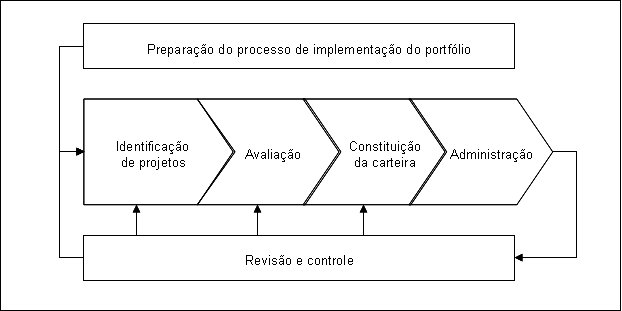
\includegraphics[width=.9\textwidth]{rabechini.jpg}
\caption{As seis dimensões do modelo de \cite{rabechini}}
\label{fig:exampleFig1}
\end{figure}

Nas rodadas de avaliação será possível estabelecer as informações de cada projeto e assim apresentar ao final informações que serão utéis para a análise 
preliminar do portfolio. Nessa dimensão um aspecto importante que deverá ser levado em conta serão as ``linhas de corte'' para os projetos, pois nesse 
momento já é possível identificar as barreiras de cada projeto individualmente. Ou seja, ao término das avaliações os projetos que ainda estão presentes 
serão os candidatos para a formação do portfolio.

A próxima dimensão, constituição da carteira, tem o intuito de estabelecer um plano de gerenciamento de portfolio. O estabelecimento de prazos é 
recomendado por \cite{clark}, prazos estes que devem ser de até um ano para alocação de recursos. 

Neste modelo é considerado que a dimensão atual deverá também ser precedida de um plano agregado do portfolio, pois nessa dimensão o aspecto de maior 
importância deve-se a observação de que neste momento serão selecionados os novos projetos que farão parte do portfolio e haverá então a disputa pelos 
recursos disponibilizados pela organização.

Na quinta dimensão, administração, constituiu-se a partir do modelo de \cite{crawford} quando esse se refere ao aspecto do gerenciamento. Os elementos 
inerentes a esta dimensão são: o controle dos recursos aos diversos projetos em curso, o acompanhamento do ciclo de vida, projeto a projeto, os custos e 
cronogramas financeiros e a qualidade do portfolio. 

Além destes elementos, nesta dimensão, espera-se que os interessados possam administrar as competências dos recursos humanos através de capacitação, 
treinamentos e coaching, quando necessário, uma vez que o sucesso da carteira depende do desempenho destes.

Ao final, temos a sexta dimensão, que diz respeito a revisão e controle. Tendo em vista que os projetos já foram selecionados, já existe a gerência do 
portfolio, cabe ao gerente de portfolio revisar o mesmo e acompanhar o desenvolvimento dos projetos. A metodologia para o acompanhamento pode ser através 
de reuniões com os gerentes de projetos ou alguma outra forma intituída pela organização. Cabe aos gerentes de projeto fornecer segundo a metodologia de 
gerência de projetos adotada pela organização, os indicadores de andamento de cada projetos

A partir daí, o gerente de portfolio será capaz de tomar decisões sobre a constituição do portfolio.

\section{O padrão apresentado pelo PMI}
Em sua segunda edição do padrão para o gerenciamento de portfolio, o PMI apresenta uma a descrição de conhecimentos e práticas de gerenciamento de 
portfolio aplicavéis e de reconhecida utilização. O padrão apresentado baseia-se no estabelecimento de processos que deverão possuir uma sequência lógica 
de realização e agrupamento por similaridade de função, além de serem divididos por áreas de conhecimento. \cite{sppm}

No modelo apresentado pelo PMI são definidos grupos de processos para o gerenciamento, os grupos aqui são definidos como de alinhamento e de monitoramento
e controle. 

Os processos do primeiro grupo, alinhamento, são os responsáveis por disponibilizar as informações, levando em consideração as metas traçadas 
no planejamento estratégico, é responsável ainda pelo estabelecimento de regras para avaliar seus componentes. São determinados como os componentes serão 
identificados, categorizados, avaliados, selecionados e incluídos no portfolio.

Já o segundo grupo, monitoramento e controle, fica responsável por reunir as atividades necessárias asseugrando que o portfolio esteja com um desempenho 
geral suficiente, fazendo assim com que seja possível atingir as metas traçadas no planejamento estratégico. Neste grupo, os processos serão responsáveis
por revisar periodicamente os indicadores estabelecidos e verificar os benefícios que os componentes do portfolio estão agregando a organização.

\begin{figure}[H]
\centering
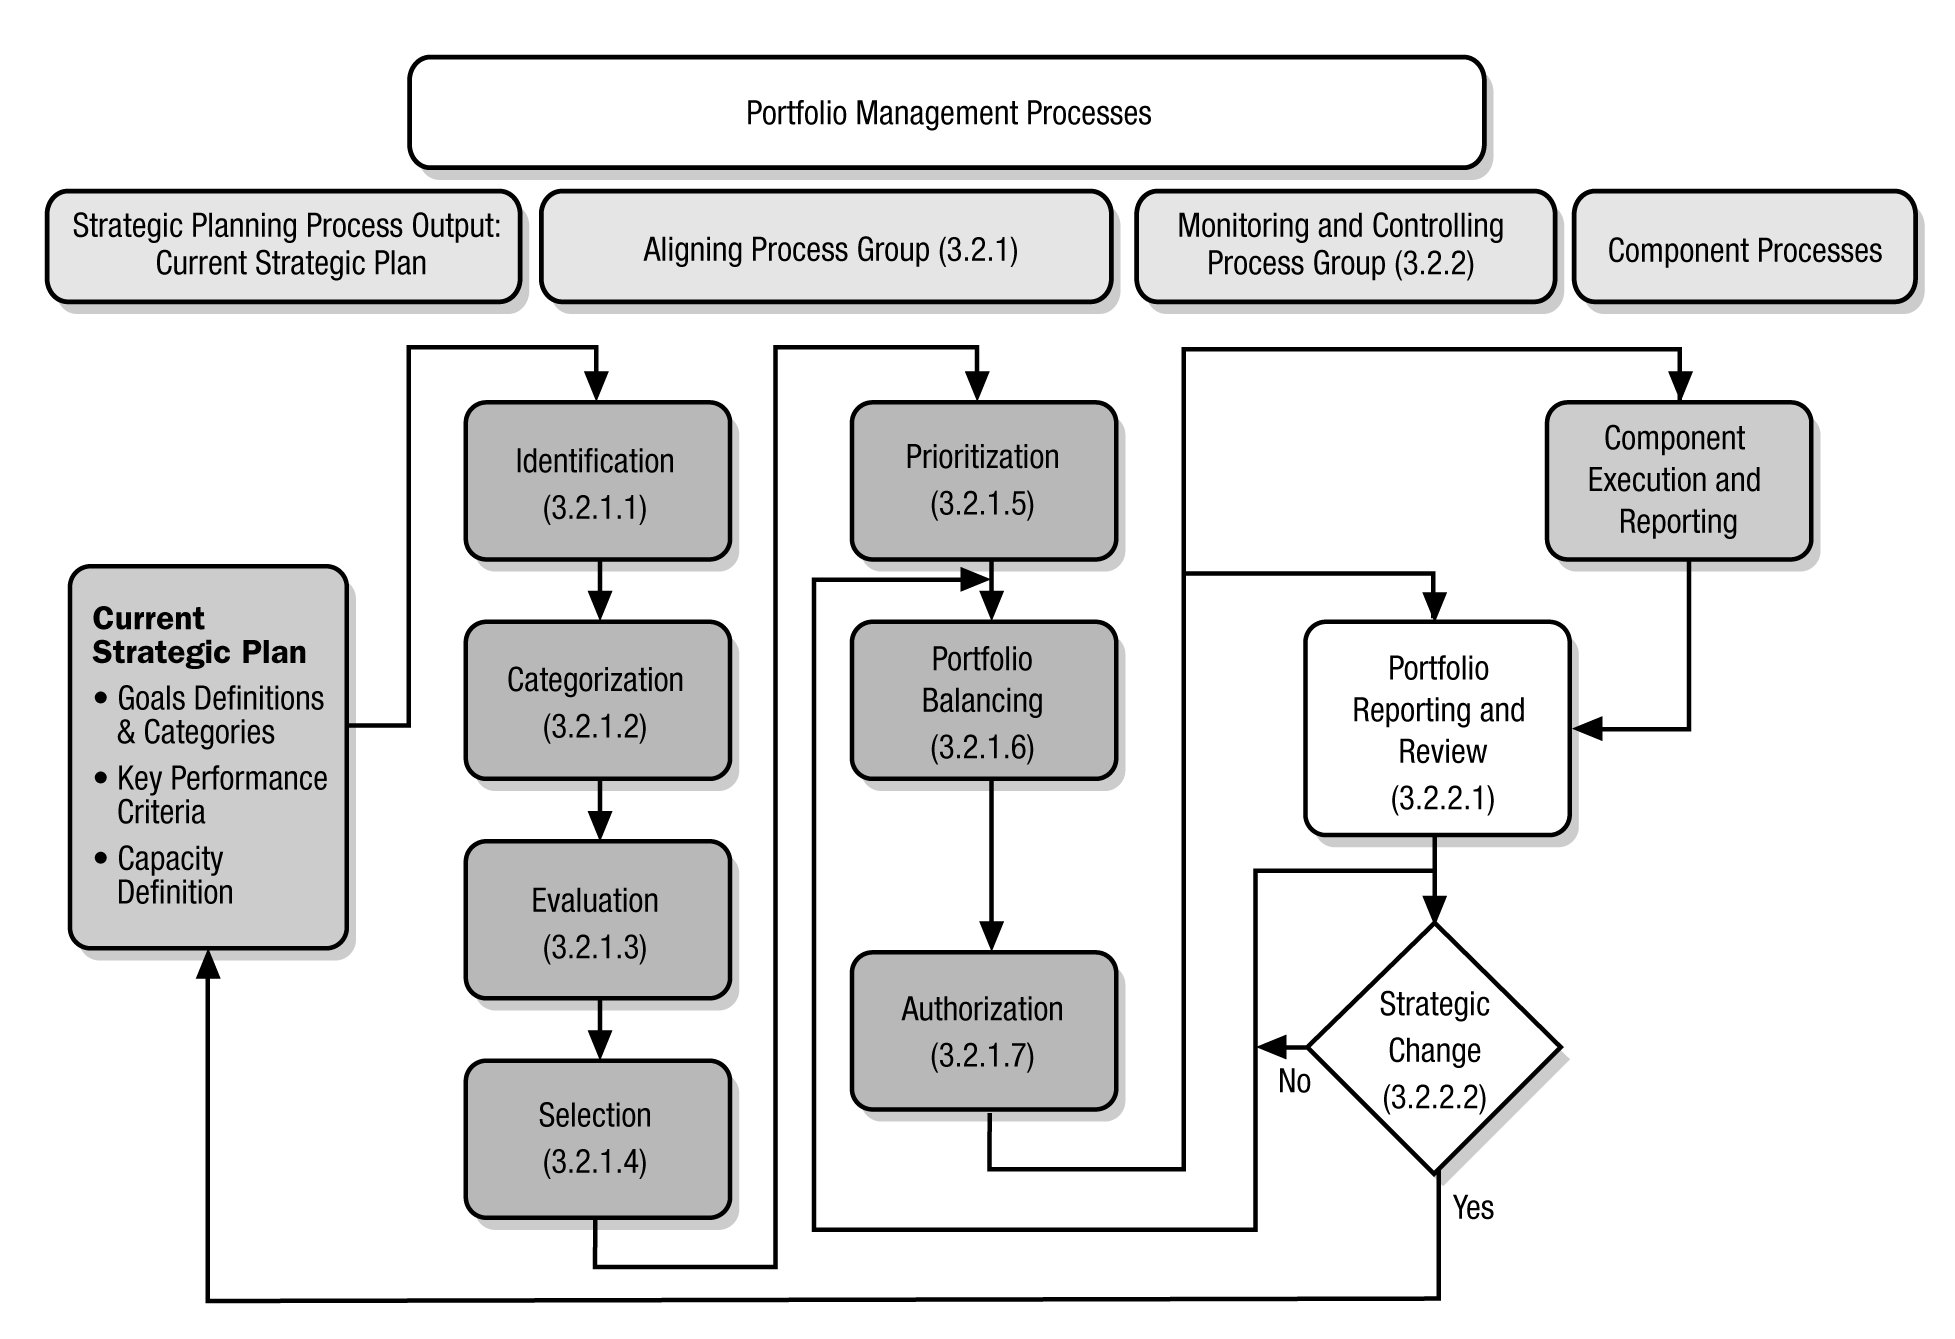
\includegraphics[width=.9\textwidth]{modelo_pmi.jpg}
\caption{Processos do gerenciamento de portfolio \cite{sppm}.}
\end{figure}

Além da divisão dos processos em grupo, o padrão apresentado pelo PMI também divide os processos em áreas de conhecimento: a área de governança de 
portfolio e a de gerenciamento de riscos.

A primeira área incluirá os processos utilizados para a seleção e investimento no portfolio, o monitoramneto e o controle dos investimentos realizados, 
a comunicação de decisões referentes a esses investimentos e a segurança de que os mesmos continuem alinhados ao planejamento estratégico da organização.

A área de conhecimento de gerenciamento de riscos diz respeito à análise de condições ou eventos que, uma vez ocorridos, possam causar efeitos positivos 
ou negativos a pelo menos um objetivo estratégico do portfolio. 

O objetivo da gestão de riscos no portfolio de projetos de uma organização é maximizar a probabilidade ou o impacto de eventos positivos e minimizar 
esses mesmos fatores, uma vez que possam influenciar negativamente o portfolio \cite{sppm}.

\begin{figure}[H]
\centering
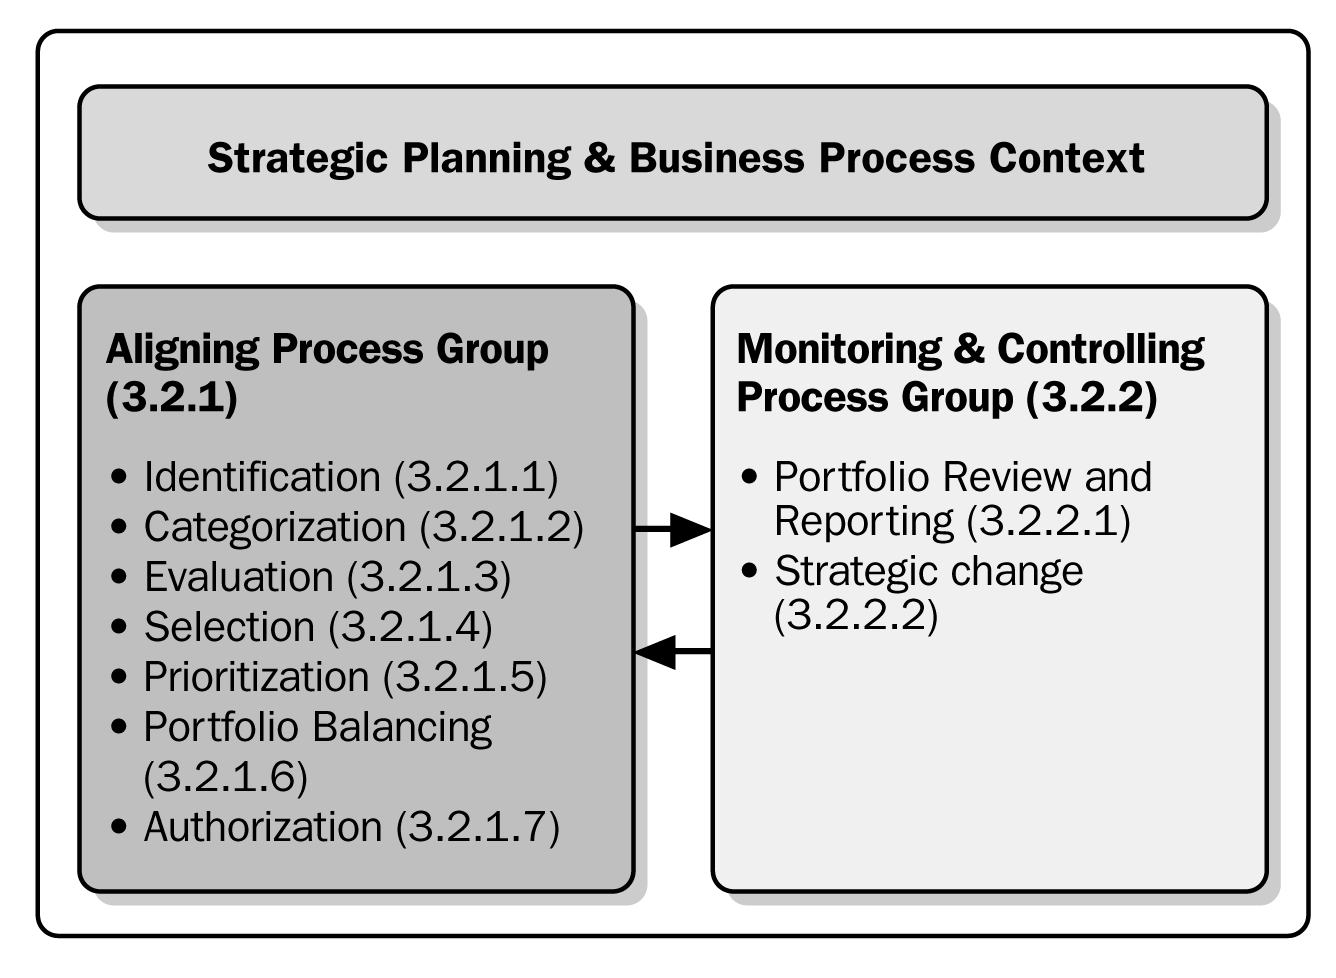
\includegraphics[width=.9\textwidth]{areas_conhecimento_pmi.png}
\caption{Áreas de conhecimento do gerenciamento de portfolio \cite{sppm}.}
\end{figure}

\section{Proposto}
Os principais modelos estudados tomam como base métodos financeiros para a tomada de decisões, e somam a estes outras ferramentas bem comuns para seleção 
de projetos. Dentre as quais cita-se: estratégia de negócio, no que diz respeito a alocação de recurso, os já supracitados métodos financeiros (Roi, NPV,
RONA), diagramas de bolha ou mapas, modelos de pontuação e check list. A partir das informações coletadas, decidiu-se também pela combinação destes 
``critérios'', sem que um ou outro acabe priorizado.

Partindo deste presuposto, cabe ao alto escalão da organização, diretores e executivos, a escolha do critério primordial. Ou seja, não dita-se a ordem 
espera-se que ao longo do processo seja possível de forma natural determinar qual a prioridade organizacional, fazendo assim com que esta seja o guia para 
as saídas do portfolio. São determinadas quatro macro fases, nas quais o portfolio passa a ser delineado, até que por fim este possa ser visualizado através 
de sua WBS ( Work Breakdown Structure ). Ao término do processo informações primordiais estarão dispostas de forma a privilegiar a visibilidade das 
definições de acordo com sua importância.

A figura abaixo apresenta o contexto onde o responsável será a diretoria executiva da organização, essa deverá considerar as metas organizacionais 
definidas e a partir destas determinar os índices a serem utilizados para a seleção de projetos. Em seguida defini-se o perfil do portfolio, ou seja, a 
orientação do mesmo. Após essa definição passa-se a etapa onde o encarregado será o gerente de portfolio, tendo esta sido terminada o portfolio retorno 
a direção executiva que deverá considerar se o mesmo atende os objetivos da organização ou não.

\begin{figure}[H]
\centering
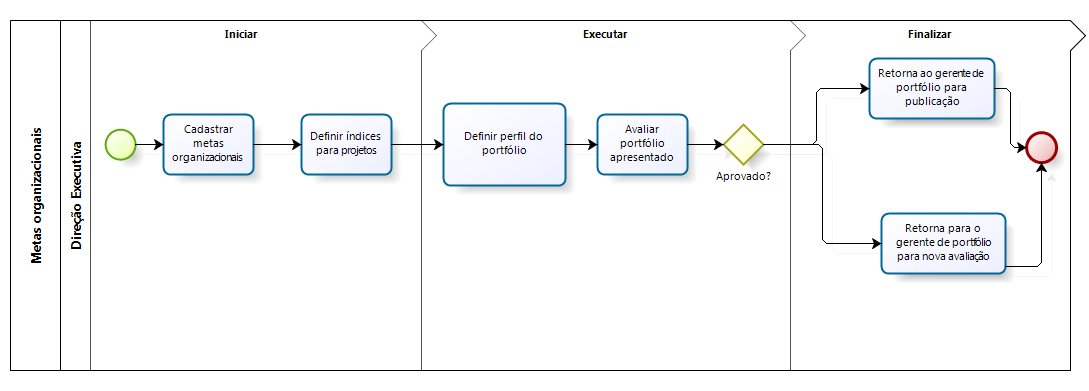
\includegraphics[width=.9\textwidth]{DirecaoExecutiva.png}
\caption{Gráfico do exercício 1.3.}
\end{figure}

Na segunda etapa o gerente de projetos, podendo ou não trabalhar em conjunto com o gerente de portfolio, deverá selecionar os projetos. Descarta-se 
aqueles que apresentam-se inteiramente fora dos padrões, considerados inviáveis ou os que não estão em andamento há algum tempo. Ou seja, a partir daqui 
trabalha-se apenas com projetos que podem ser apresentados na saída final, fase essa que deverá ser retomada sempre que um dos projetos for encerrado ou 
novos surgirem. De forma que a saída dessa etapa, lista de projetos da organização, apresente-se sempre consistente. A figura a seguir ilustra tal 
processo.

\begin{figure}[H]
\centering
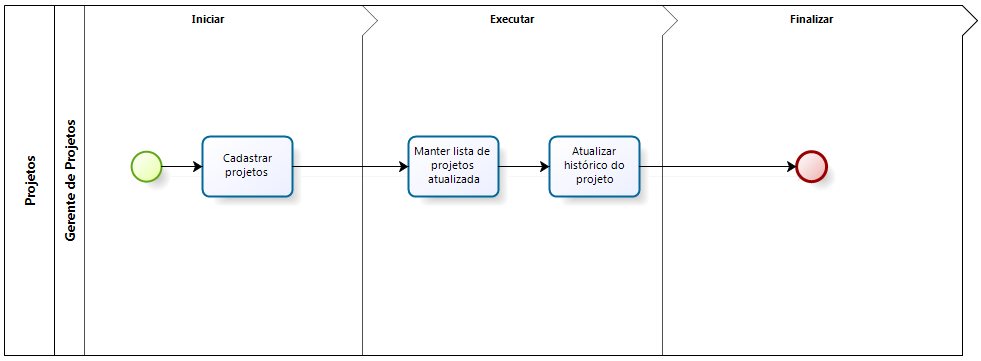
\includegraphics[width=.9\textwidth]{Projetos.png}
\caption{Processo definido para o gerente de projetos.}
\end{figure}

Com as duas primeiras fases encerradas pode-se dar início a terceira etapa, pontuação, neste momento acontece o alinhamento da estratégia organização 
aos projetos. Pois estes deverão ser analisados e pontuados de acordo com a lista de critérios apresentada pela organização. Terminada a pontuação 
determina-se quais são os principais projetos e a lista de prioridade geral destes. Etapa essa chamada de balanceamento, onde todos são dispostos de 
forma a atender o critério principal do portfolio. Sendo a saída aqui as informações referentes a quais projetos devem estar em execução, quais devem 
receber maior atenção, e assim por diante, de acordo com o que se espera do portfolio.

Na etapa final, apresenta-se a WBS supracitada, sendo possível observar o estado de cada projeto e as informações inerentes a este. Dentre as informações
pode-se citar: status, recursos, riscos, demanda, maturidade, e tantos outros quanto se desejar. Tais informações devem ser apresentadas ao alto escalão 
da organização que deverá aprovar ou não o arranjo apresentado, é importante relembrar que a escolha aqui não diz respeito a um ou outro ponto e deve-se 
observar as informações como um todo, sem que um ou outro critério possua maior influência. 

\begin{figure}[H]
\centering
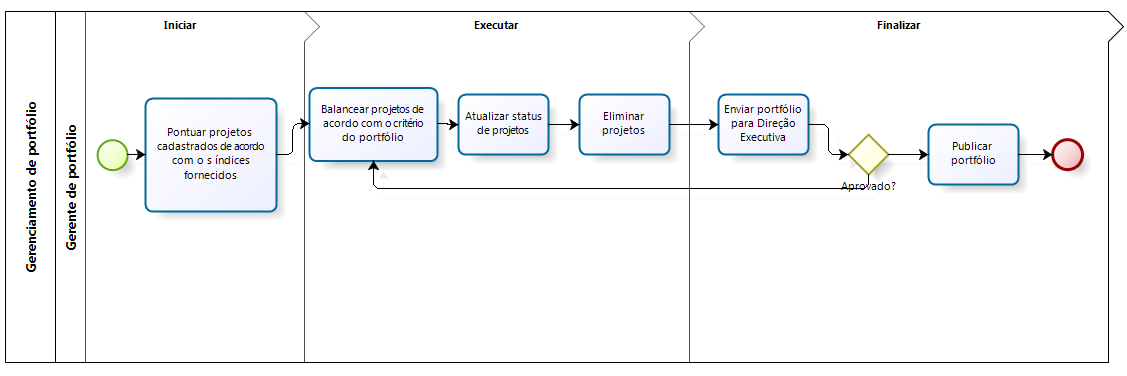
\includegraphics[width=.9\textwidth]{GerenciaPortfolio.png}
\caption{Processo definido para o gerente de portfolio.}
\end{figure}

A figura acima ilustra as etapas relativas as decisões inerentes ao portfolio em si, sendo finalizada com este sendo apresentado e aceito pela direção 
executiva da organização, assim o mesmo passa a ser o regente das etapas de desenvolvimento, assim como deverá ser utilizado para o controle e 
apresentação junto a membros internos e externos interessados nas formas de gestão da organização. Pela forma como este é apresentação, uma árvore de 
projetos contendo informações pertinentes, a organização passa a ter maior transparência e visibilidade de sua carteira de trabalho.

\chapter{Conclusão}

\begin{thebibliography}{99}
  \bibitem{archer}{ARCHER, N.P.; GHASEMZADEH, F. An integrated framework for project portfolio selection. International Journal of Project Management. v.17, n.4, p.207-216, 1999.}
  \bibitem{rodolfo}{BARROS, Rodolfo Miranda de}
  \bibitem{atila}{BELLOQUIM, Atila, Arquitetura Corporativa e Gestão de Portfolio de Projetos, Acessado via: http://www.gnosisbr.com.br/arquitetura-corporativa-e-gestao-de-portfolio-de-projetos.html, último acesso Março 2011}
  \bibitem{catelli}{CATELLI, Armando. Controladoria - Uma abordagem da Gestão Econômica - GECON. São Paulo: Atlas, 1999.}
  \bibitem{cooper}{COOPER, R. G., EDGETT, S. J. and KLEINSCHMIDT, E. J., Portfólio Management for New Products, 2dn edn,Perseus Publishing, NY, 2001}
  \bibitem{cooper2}{COOPER, R. G., Edgett, S. J. and Kleinschmidt, E. J., Project Portfolio Management in New Product Development: Results of a Industry Practices Study, Product Development Institute, ON, Canadá, 2001.}
  \bibitem{crawford}{CRAWFORD, J. K. The Strategic Project Office: a guide to improving organizational performance. New York: Marcel Dekker, 2002.}
  \bibitem{dinsmore}{DINSMORE, Paul Campbell. Transformando Estratégias Empresariais em Resultados Através da Gerência por Projeto. Rio de Janeiro: Qualitymark Ed.,1999. 284p.}
  \bibitem{artigo}{Gestão de Portfólio: o desafio do alinhamento estratégico}
  \bibitem{johnson}{JOHNSON, G., Scholes, K., Exploring Corporate Strategy: Text and Cases, Prentice Hall, Hertfordshire, UK.}
  \bibitem{kaplan}{KAPLAN, Robert S., NORTON, David P., Organização Orientada para Estratégia: Como as Empresas que Adotaram o Balanced Scorecard Prosperam no Novo Ambiente de Negócios. Rio de Janeiro, Campos, 2000.}
  \bibitem{levine}{LEVINE, H.A. Project Portfolio Management: A practical guide to selecting projects, managing portfolios, and maximizing benefits. 1. ed. New york: John Wiley \& Sons, 2005. 560p}
  \bibitem{martino1}{MARTINO, J. Apostila do curso ministrado no IPT – Instituto de Pesquisas Tecnológicas do Estado de São Paulo, 1993a.}
  \bibitem{martino2}{MARTINO, J. Tecnological forescasting for decision making. 3 ed. New York, Mc Graw-Hill, 1993b.}
  \bibitem{mcfarlan}{McFARLAN, W. E. Portfolio approach to information systems. Harvard Business Review, v. 59, n. 5, p. 142-150, Sep./Oct. 1981.}
  \bibitem{ricardo}{MOREIRA, Ricardo, Governança de TI: Um comparativo entre Cobit e ITIL}
  \bibitem{mps}{MPS.BR: Melhoria do Processo de Software Brasileiro – Guia de Implementação – Parte 2: Fundamentação para Implementação do Nível F do MR-MPS }
  \bibitem{sppm} {Standard of Portfolio Management}
  \bibitem{pmbok}{PMBOK - PMI (Project Management Institute), "Project Management Body of Knowledge", PMI, 2000 / 2008.}
  \bibitem{porter1}{PORTER, M. E. How Competitive forces shape strategy. Harvard Business Review, p. 137-145, Nov./Dec., 1979.}
  \bibitem{porter2}{PORTER, M. E. What is strategy? Harvard Business Review, p. 61-78, Nov./Dec. 1996.}
  \bibitem{prahalad}{PRAHALAD, C.K. A Competência Essencial. HSM Management, p.6-11, Mar-Abr 1997.}
  \bibitem{prahalad2}{PRAHALAD, C.K. Em Busca do Novo. HSM Management, p.6-12,Mar-Abr 1998.}
  \bibitem{rabechini}{RABECHINI JR, Roque; MAXIMIANO, Antonio C.A.;; Martins, Vergilio A.. A adoção de gerenciamento de portfolio como uma alternativa gerencial: o caso de uma empresa prestadora de serviço de interconexão eletrônica. Revista Produção, v. 15, n. 3, p. 416-433, 2005.}
  \bibitem{rockart}{ROCKART, J. F. Chief Executives define their own data needs. Harvard Business Review, v. 57, n. 2, p. 81-92, Mar./Apr. 1979.}
  \bibitem{sandra}{SANTOS, Sandra Sergi, Gestão de TI através de Portfólios}
  \bibitem{sanvicente}{SANVICENTE, Antonio Z., SANTOS, Celso da Costa.. Orçamento na Administração de Empresas: planejamento e controle. São Paulo: Atlas, 2000.}
  \bibitem{clark}{WHEELWRIGHT, S. C.; CLARK, K. B. Managing new product and process development. New York: Free Press, 1993.}
\end{thebibliography}

\end{document}
